% Local draft build (no mnras.cls required): latexmk -pdf draft_article.tex
\documentclass[11pt]{article}
\usepackage[margin=2.4cm]{geometry}
\usepackage{graphicx}
\usepackage{amsmath}
\usepackage{booktabs}
\usepackage[table]{xcolor}
\usepackage[round]{natbib}
\usepackage[hidelinks,
  pdftitle={A pilot-informed F-statistic detector for digital television
    in CHIME baseband data},
  pdfauthor={Dylan J. Gormley and Kevin Bandura}]{hyperref}
\usepackage{amssymb}
\usepackage{placeins}
% CM has no Type 1 TS1 companion here; keep the bullet in CMSY so the
% PDF stays free of Type 3 bitmap fonts (RASTI preflight).
\renewcommand{\labelitemi}{$\bullet$}
\emergencystretch=2em
% MNRAS-class conveniences used in the body:
\providecommand{\la}{\lesssim}
\providecommand{\ga}{\gtrsim}
\graphicspath{{figs/}}

\newcommand{\gpuslot}[2]{\begin{center}\fcolorbox{red}{red!4}{\parbox{0.94\linewidth}{\small\textcolor{red}{\textbf{[GPU slot -- Runbook #1]}} \small #2}}\end{center}}
\newcommand{\gpuval}[1]{\textcolor{red}{\textbf{[#1]}}}
% Author-input slots (blue): items only author can resolve -- see REFEREE_TRIAGE memo
\newcommand{\needsdylan}[1]{\textcolor{blue}{\textbf{[TODO:} #1\textbf{]}}}

\title{A pilot-informed F-statistic detector for digital television\\
in CHIME baseband data\\
\large\textcolor{red}{DRAFT --- article-class build; submission uses main.tex (MNRAS/RASTI class)}}
\author{Dylan J. Gormley and Kevin Bandura (WVU)}
\date{Draft of \today}

\begin{document}
\maketitle

\begin{abstract}
Digital television occupies much of the 470--608\,MHz band,
corresponding for 21\,cm intensity mapping to the redshift range
$1.34 < z < 2.02$. ATSC 8-VSB emission fills its 6\,MHz allocation with
noise-like symbols, and current CHIME analysis masks affected data with
statistically triggered, allocation-wide rules at visibility cadence. We
present a complementary per-frame approach keyed to the one deterministic
feature of the 8-VSB signal, the pilot tone: a quantized-weight
F-statistic from three int4 matched filters in the pilot-bearing coarse
channel, evaluated exactly in integer arithmetic, designed to gate
the station's full allocation. Synthetic characterization with a
bit-exact CPU reference lies within $\approx$0.5\,dB of ideal detection
statistics at the audited per-trial dimensionality, and
frequency-offset capture loss matches the
$\mathrm{sinc}^2$ prediction; headline thresholds await deployment-scale
regeneration. Applied to 77\,423 archived CHIME
baseband events spanning 7.6\,yr, the measured null-core zero points
agree with the analytic prediction to a few parts in $10^{3}$, consistent
with the ideal independent-row core width, with a five-channel family of
static offsets associated with reference-bin geometry. Detection rates
are non-stationary --- transitions consistent with the 2020
spectrum-repack window, plus rate collapses, onsets, and multi-year rises
--- sampled rates changed substantially between epochs separated by
order-year intervals. A retrospectively motivated candidate three-arm mask, built from exact
fixed-point compares, measures 39 per cent
retention of pilot-channel frame-time (38 per cent deployment-eligible
after a recovery-ineligibility rule masks two calibration-refused
channels), with the kept power
tail clipped at the veto threshold by construction; achieved-cleanliness
measurements are pending.

\end{abstract}

\section{Introduction}
\label{sec:intro}

The 21\,cm line redshifted into the 400--800\,MHz octave is the foundation
of the CHIME cosmology programme \citep{chang2008baryon, chime2022overview,
chime2023detection, chime2025autopower}: baryon acoustic oscillations
imprinted on large-scale structure at $0.8 \la z \la 2.5$ are measured
statistically from maps whose noise must integrate down over thousands of
hours. Terrestrial transmitters
do not integrate down. The most structured and most persistent of them is
digital television: the post-repack ATSC allocation places up to 23 6\,MHz
stations across 470--608\,MHz, and each 8-VSB signal fills its allocation
with noise-like symbol power. For 21\,cm work that band is not incidental
--- it maps to $1.34 < z < 2.02$, the high-redshift half of the CHIME BAO
range.

The 23 post-repack allocations blanket the entire 470--608\,MHz slice, so
what is at stake is not a sliver of band but 138\,MHz of frequency--time
exposure. At the telescope, however, the received 8-VSB symbol shelf from
these trans-horizon paths generally sits far below the per-channel thermal
floor; the detectable feature is the pilot tone, which concentrates
$\approx 7$ per cent of station power into a fraction of one 3\,kHz fine
bin, standing $\approx 21$\,dB above the shelf's spectral density
(Section~\ref{sec:shelfconv}). Detection therefore lives in the 23
pilot-bearing 390.625\,kHz coarse channels (8.98\,MHz), while the mask each
detection implies extends across the station's full 6\,MHz allocation
(Section~\ref{sec:whyframes}). Current CHIME analyses attack the problem
with dynamic, statistically triggered masks in the post-correlation
flagging tradition \citep{offringa2010sumthreshold, offringa2012aoflagger}
--- including a dynamic DTV rule that evaluates anomalous-bin occupancy
within each 6\,MHz allocation and masks the entire allocation for that
time sample when more than half its bins trigger, at a per-bin threshold
matched in false-positive rate to the single-sample flagging, alongside radiometer
variance tests, fringe-rate filtering, delay-spectrum filtering, and
static lists, applied aggressively at visibility cadence
\citep[Appendix~A]{chime2025autopower}; see also
\citet{rafieiravandi2023rfi} and \citet{taylor2019kurtosis} --- which
protect the science by discarding exposure: over their 94 nights of
observation, these methods excise 65.6 per cent of night-time data
across the full 400--800\,MHz band, and 38.7 per cent within the
608.2--707.8\,MHz analysis sub-band --- a band that sits entirely above
the DTV allocations. A DTV-band-only masking cost is not separately
reported; the Phase-2 comparator emulation
(Section~\ref{sec:validation}) is designed to measure it directly. Tropospheric propagation over the
long paths between the telescope and the transmitter population makes
``present'' a strongly time-varying property; a signal-keyed per-frame
detector is built to track it at the correlator's native cadence.

This paper develops, validates, and applies a complementary alternative:
per-frame \emph{detection} keyed to the one deterministic feature the 8-VSB
standard provides, the pilot tone \citep{atsc_a53}. The pilot is a CW
carrier 309.44\,kHz above the lower edge of each 6\,MHz allocation,
transmitted whenever the station radiates, at a fixed fraction of station
power. Pilot sensing of DTV is well developed in the cognitive-radio
white-space literature \citep[e.g.][]{hwang2013dtv}, and faint DTV has been
identified in 21\,cm data by subtraction-based statistics
\citep{wilensky2019ssins}; within CHIME, complementary approaches include
spectral-kurtosis excision \citep{taylor2019kurtosis}, real-time intensity
masking \citep{rafieiravandi2023rfi}, and ancillary-antenna monitoring
\citep{metzger2026ancillary}. What this paper contributes is an
alternative implementation and characterization along axes the current
masks do not occupy: a signal-keyed (rather than anomaly-triggered)
statistic, implemented \emph{exactly} in CHIME's native int4 baseband
arithmetic per 41.94\,ms correlator frame, upstream of the
visibility-cadence masks, designed for low-overhead real-time deployment,
and calibrated on-sky over multiple years with automatic
calibration-quality flags. Whether it \emph{improves} on the current
masks --- sensitivity on weak DTV at matched clean-data rejection, at a
common cadence --- is the planned Phase-2 measurement
(Section~\ref{sec:validation}). A
detector that measures the pilot measures the station: frames in which no
pilot is detectable are candidates for recovery, with the retention
statistics of Sections~\ref{sec:shelfconv} and \ref{sec:implications}
quantifying what non-detection leaves behind.

Our contributions are:
(i) a quantized-weight F-statistic detector for the pilot, computed from
three int4 matched filters inside a single coarse channel, exact in integer
arithmetic and designed for low-overhead real-time deployment
(Section~\ref{sec:method});
(ii) a synthetic characterization of its detection curves against a
bit-exact CPU reference, with the packed-int4 path consistent with a
matched full-precision control (crossing differences $-0.06$ to
$-0.02$\,dB; all 95 per cent intervals contain zero, the widest being
$[-0.24, +0.12]$\,dB) and a generator startup transient that mimicked
a $0.3$--$0.7$\,dB pilot deficit (steady-state pilot within
$0.14$\,dB of nominal; stationary-span retrim applied; sweep
regeneration pending)
(Section~\ref{sec:validation});
(iii) measured on-sky null-core ($\mathcal{H}_0$) zero points from
339\,196 frames spanning 7.6\,yr,
including a reference-geometry association for the per-channel offsets and
a falsified physics-based alternative (Section~\ref{sec:zeropoints});
(iv) a phenomenology of the detection tails --- common-mode, temporally
clustered, and dominated on multi-year timescales by rate transitions
consistent with transmitter-side events including the 2020 spectrum repack
(Section~\ref{sec:survey});
(v) a retrospectively motivated candidate operating point (a
three-arm mask) that retains
39.1 per cent of pilot-channel frame-time as its measured retention,
with a documented recovery-ineligibility rule (null-core refusal
$\rightarrow$ fully masked; 2 of 23 channels) yielding 38.0 per cent
deployment-eligible --- a
preliminary eligibility projection of $\approx 52.5$\,MHz allocation-wide
--- with a residual-power budget whose floor measurement is pending
(Section~\ref{sec:operating});
and (vi) a deployment path into the CHIME real-time system in which the
F-band arms amount to a per-channel constants swap in an existing integer
compare, alongside small new veto, broadcast, and alignment components
(Section~\ref{sec:implications}).

Throughout, values that await the production-GPU runs are marked in red
with the runbook phase that produces them, and remaining author-input
items are marked in blue. Other numbers carry one of three provenance
types --- independently recomputed arithmetic, synthetic/testbench
results, and archive-derived empirical values --- with two completion
gates: the deployment-scale regeneration of
Section~\ref{sec:synthetic}, and the GPU runs. Unless independently
regenerated here, archive-derived empirical values are provisional.

\section{The ATSC pilot and the detection problem}
\label{sec:pilot}

\subsection{Pilot structure}

ATSC 8-VSB transmits a suppressed-carrier vestigial-sideband signal whose
data symbols occupy the 6\,MHz allocation with a flat, noise-like spectrum.
The standard adds a small in-phase DC offset before modulation, producing a
CW pilot at $f_{\rm pilot} = f_{\rm lower\ edge} + 309.44$\,kHz,
approximately 11.3\,dB below the average data power \citep{atsc_a53} ---
about 7 per cent of total station power, delivered in a bandwidth far
narrower than one of our 3\,kHz fine bins. The pilot is the only
narrow-band deterministic feature of the emission, is required for receiver
lock, and is transmitted whenever the station is on air. Detecting it is
therefore operationally sufficient for ``this allocation is active at the
telescope''; what \emph{non}-detection leaves behind is characterized
probabilistically, through the pilot-free floor measurement and retention
calibration of Sections~\ref{sec:zeropoints}, \ref{sec:shelfconv}, and
\ref{sec:implications}, rather than asserted.

\subsection{Transmitter census}

We compiled a census of 490 licensed UHF stations within 800\,km
(500\,mi) of the telescope whose allocations intersect the CHIME band
(Fig.~\ref{fig:census}). Distances range from tens to hundreds of km with no
line of sight; the paths are trans-horizon (terrain confirmation for the
17.7\,km CHKL-1 relay pending; Fig.~\ref{fig:census}), so received power
is set by
tropospheric propagation and varies by tens of dB on timescales from seconds
(scintillation and aircraft scatter) to hours (ducting) to years
(transmitter-side changes; Section~\ref{sec:survey}). Three channels carry
distinctive persistent emission, all treated as environment rather than
detector failures. On ch30 the dominant signal is CHKL-1, a Penticton
relay 17.7\,km from the telescope; on ch24 a persistent carrier sits
essentially on the nominal pilot, accompanied by a secondary carrier
$+522$\,Hz away --- still inside the target fine bin --- whose
licensing identity is unresolved (the licensed CHKL-DT/CHBC-DT channel
share emits a single carrier) and operationally irrelevant: both
channels are ordinary persistent co-channel emitters, detected and
masked most of the time (mask fractions 0.69 and 0.98 under the
analytic rule), at the cost of exposure alone; beyond the calibration
bookkeeping of Section~\ref{sec:zeropoints} and the
recovery-ineligibility rule of Section~\ref{sec:implications} they
receive no special treatment. The operationally distinct case is ch33,
whose only extracted carriers sit $3$--$4$\,kHz below nominal in the
detector's skipped guard (Appendix~\ref{app:diagnostics}): an
off-nominal pilot is DTV the mask responds to only weakly
($-17$\,dB at the measured offset). The census was
retrieved 2026 June 9. Field-strength estimates at DRAO exist for 42 of
the merged census rows (43 pre-merge) from a RabbitEars Signal Search
Map study (2026 June 9; 120-mile radius; receive height at maximum,
which effectively removes terrain blocking, so the values are upper
bounds; no propagation model); they rank CHKL-1 as ch30's dominant
occupant. \needsdylan{confirm the 17.7\,km CHKL-1 path is
terrain-shielded and say so --- it reads as line-of-sight against the
``every path is trans-horizon'' statement above.}

\begin{figure}
  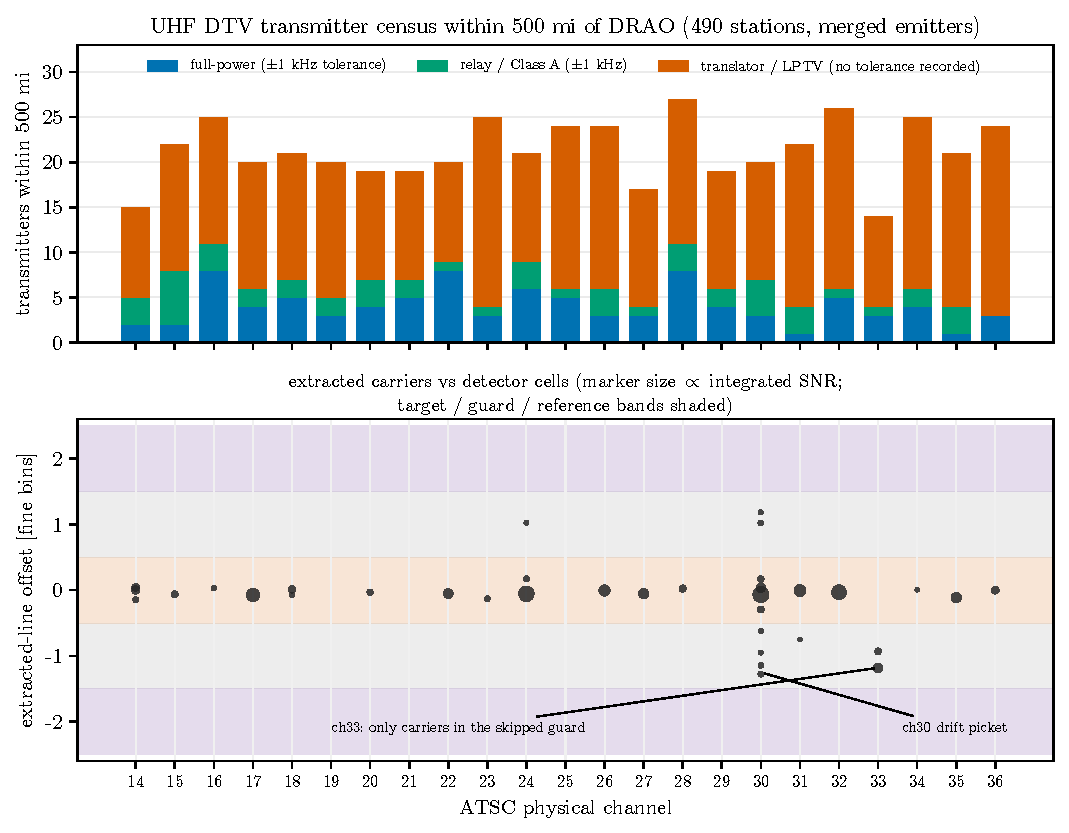
\includegraphics[width=\columnwidth]{fig1_census_context}
  \caption{Transmitter census vs the measured carriers. Top: stations
  per channel by service class within 800\,km (500\,mi) of DRAO, from
  FCC LMS and ISED data retrieved 2026 June 9 (490 on-air
  emitter-channel rows after channel-share merging, 494 $\rightarrow$
  490; off-air, analog, and ATSC~3.0 entries excluded). Full-power,
  Class~A, and relay licences carry a $\pm$1\,kHz frequency tolerance
  in the census source; translator/LPTV rows carry none. Bottom: every
  extracted carrier line against the detector-cell bands (offset from
  the nominal pilot in 3051.76\,Hz fine bins; marker size
  $\propto$ integrated SNR). The dominant carrier sits inside the
  target cell on 18 of 19 line-bearing channels; ch33's only carriers
  sit in the skipped guard --- consistent with a loosely-toleranced
  occupant (the ch33 census alone holds 11 translator/relay entries)
  --- and ch30's drift picket spans its guard
  (Section~\ref{sec:pilot}; Appendix~\ref{app:diagnostics}).
  \label{fig:census}}
\end{figure}

\subsection{Why per-frame detection, not excision}
\label{sec:whyframes}

CHIME's cosmology pipeline consumes coarse channels whole; sub-channel
spectral excision cannot help when the contaminant fills the channel.
The recoverable resource is \emph{time}: frames during which the channel is
clean. The natural unit is the correlator frame --- here 16\,384 complex
samples of one 390.625\,kHz channel across 2048 inputs, i.e.\ 41.94\,ms ---
and the natural architecture is a per-frame binary keep/mask decision made
by an exact-integer detector with an internal consistency check. Masks
aggregate trivially to any downstream cadence.

The decision is measured in one coarse channel but does not stop there. In
deployment, a pilot detection gates the \emph{entire} set of coarse
channels spanned by that station's 6\,MHz allocation ($\approx 15$
channels), because the noise-like symbol shelf accompanies the pilot across
the allocation whenever the station is received. The pilot channel is where
the decision is measured; the allocation is where it applies. The quantity reported throughout is therefore frequency--time
\emph{exposure}: measured per-frame keep fractions on the 23 pilot-bearing
channels, and their allocation-wide eligibility projection
(Section~\ref{sec:operating}). Converting a pilot excess into an implied
shelf level (Section~\ref{sec:shelfconv}) is what turns each detection into
a quantitative contamination budget for the masked and kept data alike.

\section{Method: a quantized-weight pilot F-statistic}
\label{sec:method}

\subsection{Definition}

Within one coarse channel we form, per frame and per input, matched-filter
dot products against three length-$K$ steering vectors ($K = 128$,
fine-bin width $390.625\,\mathrm{kHz}/128 = 3051.76$\,Hz): one centred on
the expected pilot bin (target $t$), and one each on reference bins $\pm 2$
fine bins away (lower $\ell$, upper $u$), with the adjacent $\pm 1$ guard
bins skipped. Powers are summed over the frame's rows (inputs $\times$
windows), giving $P_t$, $P_\ell$, $P_u$, and the detection statistic
\begin{equation}
  F \;=\; \frac{2\,P_t}{P_\ell + P_u}.
  \label{eq:fstat}
\end{equation}
Under the null hypothesis $\mathcal{H}_0$ (no pilot) the references
measure the same noise spectral density as the target and $F$ concentrates
near a computable zero point; a pilot raises $P_t$ only. (We write
$\mathcal{H}_0$ throughout to avoid collision with the Hubble constant.
The statistic is an F-ratio in the classical sense --- a ratio of summed
powers, cousin to the multitaper harmonic F-test for a line in noise
\citep{thomson1982spectrum} --- and is unrelated to the gravitational-wave
$\mathcal{F}$-statistic.) The $12.2$\,kHz total span of the three bins makes the
statistic immune to broadband gain and to any common-mode power change ---
by design and, as Section~\ref{sec:survey} shows, in practice to the level
set by frequency-selective propagation across that span.

\subsection{Quantization and the exact integer form}

The steering vectors are quantized to int4 components and shipped as a
read-only weight bank; the detector runs on CHIME's native offset-binary
int4 baseband without rescaling. Quantization makes the target and
reference vector norms unequal integers ($\mathrm{tns} \ne
\tfrac{1}{2}\mathrm{rnss}$), so the $\mathcal{H}_0$ zero point is not 1
but the analytic
\begin{equation}
  \mu_0 \;=\; \frac{2\,\mathrm{tns}}{\mathrm{rnss}},
  \label{eq:mu0}
\end{equation}
with $\mathrm{tns} = \lVert w_t \rVert^2$ and $\mathrm{rnss} =
\lVert w_\ell \rVert^2 + \lVert w_u \rVert^2$. The mask rule ``$F > \mu_0$''
is evaluated without division as the integer compare
\begin{equation}
  P_t \cdot \mathrm{rnss} \;>\; \mathrm{tns} \cdot P_r,
  \qquad P_r = P_\ell + P_u,
  \label{eq:intrule}
\end{equation}
with all sums bounded so the products fit in unsigned 64-bit arithmetic.
Every data product records the rational threshold numerator and denominator
verbatim, so any later re-thresholding is exact rather than a floating-point
reinterpretation. Table~\ref{tab:params} collects the detector parameters.

\begin{table}
  \centering
  \caption{Detector parameters (the shipped weight-bank contract).}
  \label{tab:params}
  \begin{tabular}{ll}
    \toprule
    frame & $16\,384$ samples $\times$ 2048 parallel inputs \\
    frame duration & $16\,384/390\,625\,{\rm Hz} = 41.94$\,ms
                     (inputs simultaneous) \\
    fine transform & $K = 128$ bins of 3051.76\,Hz \\
    rows per frame & $262\,144$ (inputs $\times$ 128 windows) \\
    weights & int4 components, 3 vectors (target, ref$\pm$) \\
    reference offsets & $\pm 2$ fine bins; guards $\pm 1$ skipped \\
    statistic & $F = 2P_t/(P_\ell + P_u)$; compare eq.~(\ref{eq:intrule}) \\
    operating rule & positive excess (mask $F > \hat\mu_0$) \\
    thresholds & rational, recorded verbatim per product \\
    zero point & analytic $\mu_0$ (eq.~\ref{eq:mu0}); measured
                 $\hat\mu_0$ (Section~\ref{sec:zeropoints}) \\
    \bottomrule
  \end{tabular}
\end{table}

\subsection{Capture loss}

A pilot offset by $\delta f$ from its fine-bin centre loses
$\mathrm{sinc}^2(\delta f / 3051.76\,\mathrm{Hz})$ of captured power;
$\pm 1$\,kHz costs 1.59\,dB. Section~\ref{sec:synthetic} verifies this
prediction to $\sim$0.1\,dB, and the census shows real pilots park within a
few hundred Hz of nominal except for the off-nominal ch33 carrier
(Section~\ref{sec:pilot}; Appendix~\ref{app:diagnostics}).

\begin{figure}
  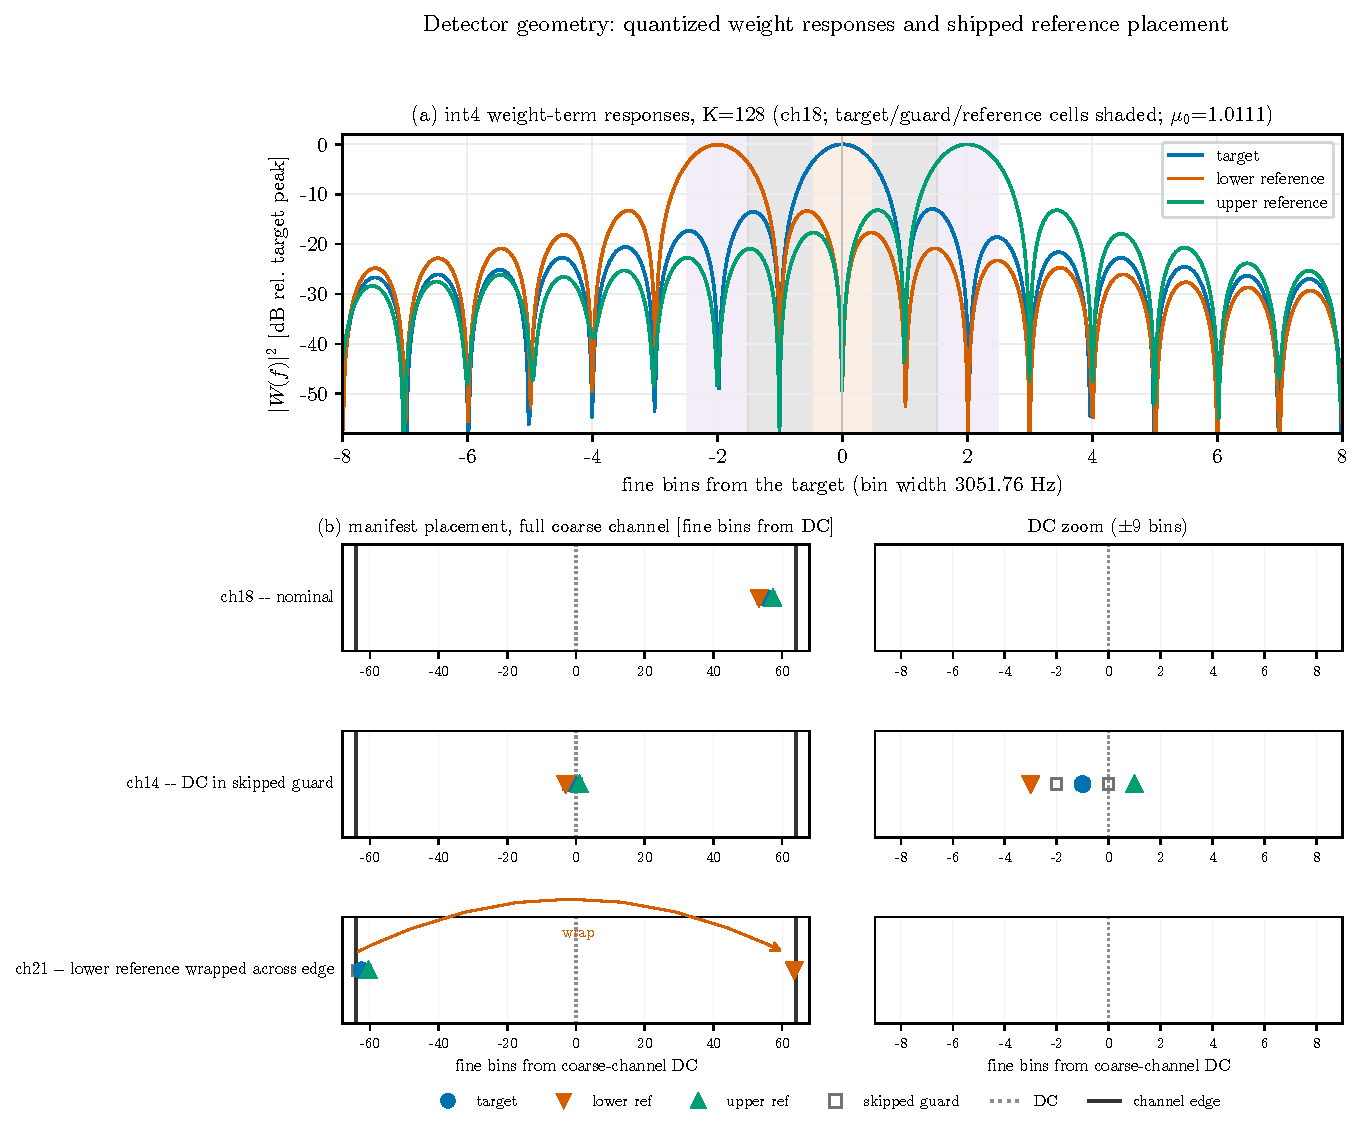
\includegraphics[width=\columnwidth]{fig2_detector_geometry}
  \caption{Detector geometry. (a) Quantized weight-term responses
  $|W(f)|^2$ with the target, skipped-guard, and reference cells shaded.
  (b) Manifest placements for the three distinct geometries that occur:
  nominal (ch18), coarse-channel DC falling in a skipped guard (ch14),
  and the lower reference wrapped across the channel edge (ch21). The
  placement rule also shifts a reference that would collide with DC;
  the closest approach in the shipped bank is 2.1 bins (ch28), so that
  branch never fires and is not drawn.
  \label{fig:geometry}}
\end{figure}

\subsection{From pilot excess to shelf power}
\label{sec:shelfconv}

The statistic is also a meter. For small excess, the fractional shift of
$F$ above the measured zero point estimates the in-bin pilot-to-noise
ratio,
\begin{equation}
  p \;\equiv\; \frac{P_{\rm pilot}}{N_{\rm bin}} \;\approx\;
  \frac{F}{\hat\mu_0} - 1,
  \label{eq:pilotexcess}
\end{equation}
and the ATSC power budget ties the pilot to the symbol shelf: with the
pilot 11.3\,dB below the data power and the shelf referenced to the full
6\,MHz allocation (the convention fixed throughout the analysis code),
the pilot stands a factor $C = 145.7$ ($+21.64$\,dB) above the per-bin
shelf spectral density, so a measured excess implies a shelf-to-noise
spectral-density ratio $\approx p/145.7$ across the station's
allocation. Equation~(\ref{eq:pilotexcess}) is an estimator, not a bound: a
signal-bearing frame can fall below $\hat\mu_0$ on a negative noise
fluctuation, so single-frame retention proves nothing. The deliverable is
probabilistic --- $P(\mathrm{retained} \mid \rho_{\rm shelf})$, the
retention probability as a function of shelf level, measured directly
from the Phase-2 real-baseband injection ladder. The conversion
constant also assumes the transmitted pilot-to-shelf ratio survives
propagation; multipath can notch pilot relative to shelf, and injection
calibrates only the relation that is injected, so propagation-induced
pilot-to-shelf decorrelation remains a separate systematic to bound.
Moreover $P(\mathrm{retained} \mid \rho_{\rm shelf})$ is an acceptance
curve, not itself a bound: it must be \emph{combined with} an
environmental shelf-level occupancy model to yield the distribution of
retained contamination --- a model that detection rates alone cannot
supply once pilot--shelf decorrelation is admitted, requiring in addition
simultaneous wideband (allocation-spanning) power information and an
explicit decorrelation prior. That distribution is the quantity that
would feed a future uncertainty-to-BAO forecast.
\needsdylan{validate the conversion constant against the Phase-2 ladder
before quoting shelf levels from real data.}

\FloatBarrier  % keep Fig. 2 inside its own section
\section{Implementation}
\label{sec:implementation}

\textit{pilot-proxy} implements the detector as a CUDA kernel operating on
packed int4 baseband with the exact compare of eq.~(\ref{eq:intrule}), and,
critically for this paper, as a bit-compatible pure-CPU reference
implementation used for all validation that does not require GPU
throughput. Products carry the full provenance needed for exact post-hoc
analysis: per-frame $P_t$ and $P_r$ as u64 integers, the rational
thresholds, weight-bank hashes, and per-unit absolute time tags.

\textit{datatrawl} supplies the archive side: storage-safe streaming of
baseband events from the CHIME archive \citep[captured by the system
described in][]{michilli2021baseband}, resumable scans with exact
(event, frame) identity, and inventory provenance. Both packages are open
source with citation metadata (see the Data Availability statement); the
detector data sheet and user guide are attached to their releases.

\section{Validation}
\label{sec:validation}

Validation follows the five recorded items of the publication plan
(dates in Appendix~\ref{app:prereg}):
synthetic detection curves (item 2), on-sky $\mathcal{H}_0$ zero point and
control
certification (item 1), injection--recovery (item 3), radiometer baseline
(item 4), and the cleaning tradeoff (item 5). Item 5's tradeoff study
motivates a candidate operating point; item
2's curves are in hand with their conventions audited against the
testbench source (Section~\ref{sec:synthetic}) and deployment-scale
regeneration pending; item 1 is complete on the survey side with its
control certification pending; items 3 and 4 await production-GPU runs
and appear as marked slots.

\subsection{Synthetic detection curves (item 2 --- conventions audited; deployment-scale regeneration pending)}
\label{sec:synthetic}

We generate a standards-chain 8-VSB waveform (the GNU Radio ATSC transmit
chain: randomizer, RS encoder, interleaver, trellis, field-sync mux, RRC
pulse shaping), add complex AWGN, channelize through the 4-tap
sinc-Hamming reference PFB, quantize to offset-binary int4 ($3\sigma$
clip), and run the bit-exact CPU reference detector at 1000 trials per
grid point over $-38 \le \mathrm{SNR} \le -24$\,dB and pilot offsets
$\{-1, 0, +1\}$\,kHz (Fig.~\ref{fig:curves}). The conventions, audited
against the testbench source, are: \emph{shelf SNR} is the DTV data-shelf
PSD averaged over the full 6\,MHz allocation relative to the noise-floor
PSD in the same band; the \emph{integrated} pilot power is 11.3\,dB below
the \emph{integrated} data-component power, so after the 6\,MHz spreading
conversion the target fine bin sees the pilot a factor $C = 145.7$
($+21.64$\,dB $= -11.3$\,dB $+ 32.94$\,dB) above the per-bin shelf
density. ($C$ is defined against the \emph{allocation-averaged} shelf
density, i.e.\ integrated data power spread over the full 6\,MHz;
against the interior-plateau density it would be 130.7.)
Two rules are characterized. \emph{The deployed positive-excess rule}
(eq.~\ref{eq:intrule}) is the operational cleaning rule: its
$\mathcal{H}_0$ ``detection'' rate is by construction the $\approx 0.5$
mask fraction, i.e.\ a false-mask probability $P_{\rm FA} \approx 0.5$
accepted deliberately (Section~\ref{sec:cleaning}), and it reaches
$P_{\rm d} = 0.9$ at $\approx\mathbf{-32.7}$\,dB per trial.
\emph{The fixed-threshold mode} is the same rational-threshold machinery
evaluated at a fixed physical level --- mask iff $F$ exceeds the F-level
a $-32$\,dB shelf implies under this mapping --- retained as a
calibration-free \emph{backup operating mode}: it requires no measured
zero point, so it can run before a null-core calibration exists or while
the mask-fraction health check flags drift. As implemented in the
testbench and as tested here, the threshold is the \emph{unnormalized}
raw-F level and the tested curve is channel 14's; the deployment
specification additionally rescales the level per channel by the
\emph{analytic} $\mu_0$ (itself calibration-free) --- a per-channel
constant that leaves each curve's shape unchanged --- because an
unnormalized common raw threshold would shift the effective midpoint by
up to 1.31\,dB across the shipped $\mu_0$ range. Its level is a recorded
testbench convention, not a derived requirement \needsdylan{if a
science-derived required sensitivity is later established, cite it here
and set the backup level from it}; at that level the backup mode reaches
$P_{\rm d} = 0.5$ at $\approx -31.8$\,dB and $P_{\rm d} = 0.9$ at
$\approx -29.1$\,dB per trial (linear interpolation on the 1\,dB grid;
fitted crossing uncertainties pending; the backup curves are archived
in the sweep summary and deliberately not drawn in
Fig.~\ref{fig:curves}, which shows the deployed rule only). Each trial is one
16\,384-sample frame of \emph{four} input streams --- $R = 512$ detector
rows, not the 262\,144 of a full 2048-input frame --- so the ideal null
width per trial is $\sqrt{1/R + 1/(2R)} = 5.4$ per cent, and every curve
in Fig.~\ref{fig:curves} is a per-512-row-trial curve.
\needsdylan{quote the crossings with fitted uncertainties rather than to
0.01\,dB on regeneration.} Both rules' curves
are monotone within Wilson 95 per cent intervals
\citep{wilson1927probable} at every offset, with transition-region
half-widths of 2.8--3.1 per cent, and the $\pm 1$\,kHz
curves shift by $+1.71$ and $+1.70$\,dB against the $\mathrm{sinc}^2$
prediction of $+1.59$\,dB, quantitatively confirming the capture
model.

Because the rule has no free parameter, the detection curve is
deterministic once the null width is calibrated, and the rule's
natural sensitivity scale is the \emph{width-crossing} SNR at which
the mean excess $Cs$ equals one null width $\sqrt{1/R + 1/2R}$:
$-34.3$\,dB per 512-row trial and $-47.9$\,dB per full 2048-input
frame ($P_{\rm d}\approx 0.84$ there by construction); every crossing
quoted in this paper is a point on that same mapping. The text quotes
the operational crossings, and Fig.~\ref{fig:curves}
serves as the \emph{model-validation instrument} across the range ---
its panel-(a) mean-excess residuals are what exposed the generator
calibration issues of this section in the first place.
Under the exact \emph{ideal independent-Gaussian benchmark} ($F \sim
\mu_0\,\mathrm{ncF}(2R, 4R, \lambda)$, $\lambda = 2RCs$ at linear shelf
SNR $s$ --- a benchmark, not the exact distribution of the packed-int4
statistic), and accounting for the raw-F threshold against the channel-14
null centre $\mu_0 = 1.00206$, the predicted crossings (backup-mode
$P_{50}$/$P_{90}$ and deployed-rule $P_{90}$) are $-32.09$,
$-29.38$, and $-33.04$\,dB against the measured $\approx -31.8$,
$-29.1$, and $-32.7$\,dB --- near-uniform offsets of $+0.27$, $+0.30$,
and $+0.32$\,dB --- while the positive-excess rate at the $-38$\,dB grid
edge agrees within the trial statistics (0.6611 predicted; 0.662
measured; $\sigma_{1000} = 0.015$). Two measurements decompose these
offsets. First, a matched full-precision control: every archived trial
records the float-weight statistic alongside the packed-int4 one, and
the float-weight crossings differ from the int4 crossings by
$-0.05$, $-0.02$, and $-0.06$\,dB, with paired-bootstrap 95 per cent
intervals of $[-0.12, +0.02]$, $[-0.10, +0.05]$, and $[-0.24, +0.12]$\,dB
--- the point estimates are small relative to the residuals, although
the widest 95 per cent interval permits a contribution as large as
0.24\,dB; quantization is disfavoured as the dominant term but not
excluded at that level. Second, waveform calibration: two committed estimators measure the
golden capture's integrated pilot-to-data ratio under different
conventions. The extended waveform audit (in the provenance bundle with
the raw 45\,000-trial records, hashes, and producing commit) reads
$12.024$\,dB from the capture's first $262\,144$ samples, with the
pilot's contribution taken from a $\pm 10$\,kHz window against a
median-shelf baseline; the pilot-trim utility's coherent projection
over the full $600\,000$-sample capture (committed
\texttt{trim\_report.json}) reads $11.830$\,dB. A four-way decomposition
(both captures audited at both spans) separates the conventions: at
fixed windowed method, extending the audit span from the capture's
first $262\,144$ to its first $524\,288$ samples moves the scalar by
$-0.43$\,dB (original) and $-0.41$\,dB (trimmed), and at the longer
span the windowed scalar sits $0.22$--$0.24$\,dB \emph{below} the
projection values. The window-summed pilot power is $0.84$\,dB higher
in the capture's second $262\,144$ samples than in its first, while
the data power changes by only $0.01$\,dB: the audit scalar is
span-dependent because the generated pilot line itself is not
stationary across the capture. A ten-block projection profile
localizes this to a generator startup transient --- the first
5.6\,ms block carries $-9.7$\,dB of the stationary pilot power and
the second $-0.4$\,dB, with the line stationary within measurement
noise thereafter and a benign $-0.07$\,Hz projection-frequency offset
(0.022\,rad total drift; coherence loss $<10^{-4}$). The single-number full-capture generator deficit is
therefore convention-bounded at $0.30$--$0.72$\,dB below the nominal
11.3 --- and the stationary-span measurement below shows it to be
transient-dominated, with the steady-state pilot $0.14$\,dB above
nominal --- while the trim's shift is convention-stable ($-0.53$\,dB by
projection; $-0.53$ and $-0.51$\,dB by the windowed method at the two
spans) and leaves the data power identical to nine significant
digits. The synthetic trials are immune to a positional systematic:
every trial channelizes the same leading $\approx$451\,000 clean
samples, and the frame-effective (window-incoherent) pilot power over
exactly that span equals the trim's full-capture projection basis to
$0.003$\,dB, so the trimmed capture presents the intended 11.30\,dB
ratio to the detector. The citable regeneration nonetheless uses a
clean protocol --- crop the capture to the stationary span the
evaluator consumes, re-estimate and re-trim \emph{that} span, audit
the same span, and regenerate the sweep from it (cropping after the
existing trim would leave the stationary pilot $\approx 0.6$\,dB
strong) --- and its calibration steps are now executed: the cropped
stationary span measures $11.164$\,dB by projection, i.e.\ the
\emph{steady-state} generator pilot sits $0.136$\,dB \emph{above}
nominal and the apparent full-capture deficit was the startup
transient diluting the mean; the retrim is a $-0.136$\,dB touch
(amplitude $\times 0.9845$) to exactly 11.300. On the stationary
trimmed capture the audit's direct and shelf-extrapolated fields agree
to $0.007$\,dB (11.404 and 11.411), collapsing the earlier estimator
spread; the residual $+0.10$\,dB audit-vs-projection gap is method
bias plus a mild residual drift within the span (the audit's default
262\,144-sample span reads the span's earlier, slightly cooler
portion). The stationary sweep regeneration is queued behind the
in-flight block. The audit's peak bin is
consistent with the generator's pilot placement within its 164\,Hz PSD
resolution; placement itself is set by the generator's mixing
parameters. Interior-shelf estimators bracket
the direct value (median-Welch 11.918, mean 12.375); an earlier
ideal-raised-cosine inference of the integrated ratio (11.446) is
superseded by the direct measurements. The offsets are therefore
dominated by the waveform/convention side: propagating even the larger
$0.72$\,dB through the composite-power normalization predicts a
$0.68$\,dB pilot-to-noise shift --- which, were nothing else different,
would move the $+0.30$\,dB offsets to $\approx -0.38$\,dB --- so the
simple amplitude story \emph{over}predicts, and the compensating
component (sample span, pilot-window baseline, band-edge conventions,
or capture model) is not yet attributed. We quote the measured
$+0.27$--$0.32$\,dB as the end-to-end calibration envelope; the
pilot-trimmed regeneration (trim applied at the projection convention:
$11.830 \rightarrow 11.300$, amplitude $\times 1.0629$, $+0.53$\,dB)
measures the amplitude component directly and is the closure step.
Measured on the trimmed capture (audit v3): the direct field reads
$11.497$\,dB --- the predicted $\approx 11.49$ (11.30 at the projection
convention plus the convention gap), reproducing the
default-span convention offset on both sides of the trim; the
shelf-extrapolated estimator reads 11.391, and the trimmed pilot sits
within 0.44\,Hz of nominal placement (the audit's coarse quality gates
also pass, but their $\pm 2$\,dB pilot-level tolerance makes them no
evidence of amplitude closure). The amplitude-closure verdict now rests on the regenerated
sweep crossings (folding a ratio into the SNR axis remains
inappropriate --- the chain does not respond to the direct ratio
alone).

Because the mean pilot excess at fixed shelf SNR is
dimensionality-independent while the null width shrinks as $1/\sqrt{R}$,
a full 2048-input frame is $10\log_{10}\sqrt{262\,144/512} = 13.6$\,dB
deeper in positive-excess sensitivity (the fixed-threshold mode's
midpoint does not move): analytically, the deployed positive-excess rule
reaches
$P_{\rm d} = 0.9$ near $-47$\,dB shelf SNR per full frame, and the
backup mode's transition at its reference level becomes essentially a
step.
\needsdylan{regenerate Fig.~\ref{fig:curves} at deployment dimensionality
(same sweep, \texttt{--num-input-streams} at the deployment value) or add
the analytic full-frame scaling to the figure, before any headline
sensitivity number returns to the abstract.}

\begin{figure}
  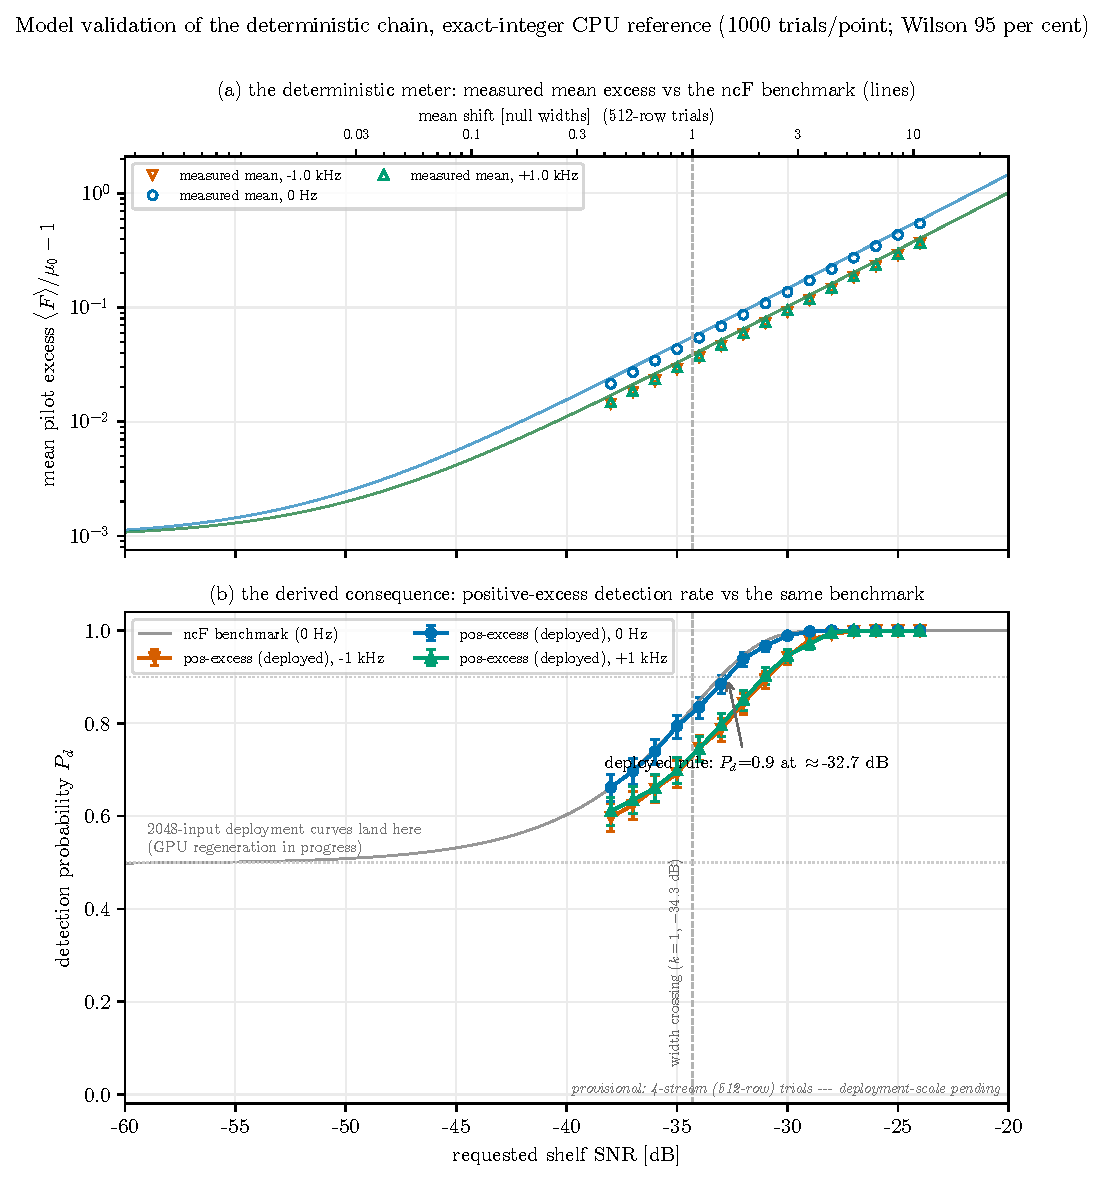
\includegraphics[width=\columnwidth]{fig3_detection_curves}
  \caption{Model validation of the deterministic chain (exact CPU
  reference, 1000 trials/point, Wilson 95 per cent; offsets 0,
  $\pm$1\,kHz). Because the positive-excess rule has no free
  parameter, both panels are predictions, not fits. (a) The meter: the
  measured mean pilot excess against the ncF benchmark lines --- the
  constant offset below the lines is the untrimmed capture's pilot
  deficit rendered directly, the calibration ledger of
  Section~\ref{sec:synthetic}; the stationary-capture regeneration
  should place the points on the lines. (b) The derived consequence:
  the positive-excess detection rate against the same benchmark (grey),
  flattening at the by-construction $P_{\rm FA}\approx 0.5$ floor.
  The fixed-threshold backup mode is deliberately not drawn (archived
  in the sweep summary; levels quoted in the text). Curves are per
  512-row trial; the 2048-input deployment curves from the GPU
  regeneration land in the annotated region.
  \label{fig:curves}}
\end{figure}

\textbf{CPU/GPU parity (Phase 1c) --- measured.} A same-seed spot check
at $-31$\,dB shelf SNR, 0\,Hz offset, channel 14, four streams (seed
20260715, 200 trials, A100, kernel v1.0.0):
$\max|F_{\rm GPU} - F_{\rm CPU}| = 0$ across all trials against both the
packed-integer and reference CPU implementations, with trial-by-trial
identical detection decisions under both rules (126/200 backup-mode;
197/200 positive-excess) and a zero rational-overflow count. The
per-trial records are archived in the provenance bundle and committed to
the public repository
(\texttt{data/provenance/parity\_gpu\_20260715seed}); the weight bank
is byte-identical between the CPU sweep and the GPU session
(sha256 \texttt{b0dce17a\ldots}). This supports CPU$\leftrightarrow$GPU
parity for exactly the tested configuration; the public CI suite is
CPU-only (its CUDA test skips without a device and exercises a single
geometry when enabled), so GPU parity across the remaining geometries
is future verification, and per-trial CPU-side $(P_t, P_\ell, P_u)$
integers are not separately archived by the current schema.

\subsection{On-sky null-core zero points (item 1 --- survey side complete)}
\label{sec:zeropoints}

Applied to the archive (Section~\ref{sec:survey}), the measured zero
points $\hat\mu_0$ --- estimated per channel by a mode-anchored iterated
median over a $\pm 6\times 10^{-3}\mu_0$ core window, with automatic trust
flags. The flags are quantitative and recorded: the measured zero point
is \emph{refused} when any of (i) the mask fraction at the analytic
$\mu_0$ exceeds 0.9 (an always-dominated channel), (ii) fewer than 15
per cent of valid frames fall within the located core window (the core
is not a population), or (iii) the located core is displaced more than
$20\times10^{-3}\mu_0$ from the analytic zero point. The specific
values are recorded conventions imported with the original study
script; no community standard prescribes them directly, but they
reduce to one interpretable criterion plus a range check. Because the
positive-excess rule masks null frames at 0.5 by construction and
strong-signal frames at $\approx 1$, a channel's mask fraction under
a null/signal mixture is $1 - 0.5 f_{\rm null}$, so the 0.9 flag is
the statement $f_{\rm null} < 0.2$; the $\pm 6\times10^{-3}$ core
window (2.5 ideal null widths) captures essentially all of a true null
population, so the 15 per cent occupancy flag is the statement
$f_{\rm null} \lesssim 0.15$ by direct count. Two flags, one
criterion --- an identifiable null subpopulation of at least
$\sim$15--20 per cent --- measured two independent ways; they catch
the overwhelming-signal failure (ch30, $f_{\rm null} = 3.4$ per
cent). The displacement flag is the independent axis, catching the
weak-but-permanent failure (ch24, whose carrier is too faint to mask
every frame but displaces the located mode): $20\times10^{-3}$ is
$\approx 1.7\times$ the
largest shift the detector geometry produces anywhere in the bank (the
ch21 wrap). The specific values do no delicate work: the observed population is strongly bimodal, with
trusted displacements topping out at $12.0\times10^{-3}$ (ch21)
against $20.4\times10^{-3}$ for the nearest refusal (ch24), and
trusted core occupancy bottoming out at 19.5 per cent (ch17) against
7.6 per cent (ch24) --- any thresholds inside those empirical gaps
select identically. The physical discriminator the flags encode is
population and sign: ch21 relocates an intact null population (88 per
cent of its frames in one core; a reference-side geometric effect,
negative by construction), whereas the refusals' positive
displacements can only be target-cell power, corroborated by the
in-cell carriers visible in the supplementary spectra. The occupancy
floor is an estimator-scope statement, not a physics one: masking a
heavily-contaminated channel while keeping a certified clean minority
is exactly the intended operation, and a channel with a \emph{genuine,
identifiable} minority null population could in principle be
calibrated by a mixture-model estimator rather than the mode-anchored
one, which necessarily locks onto the dominant clump. No such channel
exists in this archive (the occupancy gap 7.6--19.5 per cent is
empty), but that is the route by which a refused channel could be
reclaimed --- and we tested it where it looks most promising. ch30's
$F$ distribution is cleanly bimodal: 96 per cent of frames in the
located $11.7\times\mu_0$ clump, an essentially empty gap from 1.5 to
$10\times\mu_0$ (0.26 per cent), and a 3.5 per cent minority below.
The minority is 38 whole captures confined to a single off-air
interval (2019 April 6--25, plus one October day); no capture mixes
the two populations, so these are transmitter silences, not
propagation fades. Its centre lies within $1.5\times10^{-3}$ of the
\emph{analytic} zero point --- direct evidence that the refusal is
transmitter-caused, not instrumental --- but it is not a calibration
core: the within-capture width is $37\times10^{-3}$, fifteen times
the trusted-channel null width, with capture means scattered
$18\times10^{-3}$ rms in \emph{both} directions (consistent with weak
residual co-channel energy in target and reference cells once the
dominant carrier is off), occupancy 0.5 per cent against the 15 per
cent floor, and zero exposure in any epoch after 2019
(\texttt{ch30\_offair\_minority.csv}). The mixture route, applied to
the one channel that invites it, therefore confirms the refusal
rather than reversing it; retained frames on a refused channel cannot
be distinguished from sub-threshold signal leak and are not
certified. \needsdylan{corroborate the 2019 April 6--25 ch30 off-air
interval against the occupant's records (ISED; census candidate
CHKL-1) alongside the Section 6.3 lookups.}
These same flags are the membership test of the
recovery-ineligibility rule (Section~\ref{sec:implications}). The
flags partition the 23 channels cleanly: 21 yield a calibrated null
core, of
which 16 are nominal, sitting within $\pm 3.4\times10^{-3}$ of the
analytic $\mu_0$, and five form a static geometric family ($-2.2$ to
$-12\times10^{-3}$) explained bin-by-bin by reference placement; the
remaining two are refusals (Fig.~\ref{fig:zeropoints}; per-channel
diagnostics in Appendix~\ref{app:diagnostics}). The measured core width,
$\approx 2.4\times10^{-3}\mu_0$, is consistent with the ideal
independent-row width $\sqrt{1/R + 1/(2R)} = 2.39\times10^{-3}$ of a full
frame of $R = 262\,144$ rows: the on-sky null behaves like the
full-dimension statistic --- a consistency check at the quoted precision
(no width uncertainty is yet assigned) against the accounting of
Section~\ref{sec:synthetic}:

\begin{itemize}
  \item \textbf{A five-channel geometric family} of static whole-core
  shifts: $-12.0\times10^{-3}$ (ch21, lower reference wrapped across the
  coarse-channel edge), $-4.5$ (ch25) and $-3.6$ (ch28, references near the
  DC spur), $-4.2$ (ch14, DC in the skipped guard), and $-2.2\times10^{-3}$
  (ch36, band-edge roll-off).
  % NOTE: text previously said -3.7 for ch28; Table 2 says -3.6.
  % confirm against empirical_zero_points.csv (triage E2).
  Each is associated bin-by-bin with reference placement against fixed
  spectral furniture; the deployed response has not been quantitatively
  reproduced (the prototype model below fails), so the measured table,
  not a mechanism, is the calibration.
  \item \textbf{Two refusals, for different reasons}: on ch30 a nearby,
  dominant station leaves essentially no pilot-free frames (the
  measured exception: the 3.5 per cent 2019 off-air minority dissected
  above) --- the
  located mode sits at $11.7\times\mu_0$ --- so there is no
  null core to measure --- the channel is masked almost always regardless
  (Table~\ref{tab:perchannel}); on ch24 the estimator finds a modal core
  displaced $+20.4\times10^{-3}$, i.e.\ signal-elevated by the
  persistent in-cell carriers of Section~\ref{sec:pilot} --- so
  anchoring $\hat\mu_0$ there would calibrate the null against
  contamination. The estimator flags rather than fits both --- evidence
  against circularity, as is ch33's measured mask fraction of 0.528 (the
  method does not force 0.5).
  \item \textbf{A falsified physics alternative}: a deterministic
  prediction of the shifts from the 4-tap sinc-Hamming reference PFB
  prototype (aliased noise shape through the $K=128$ window) predicts
  $-1.8$ to $-4.2\times10^{-3}$ for the near-edge channels 18/29/32/35,
  where the measurement is consistent with zero, and captures only a third
  of ch21's shift (Fig.~\ref{fig:pfbpred}, Appendix~\ref{app:diagnostics}).
  The deployed F-engine coefficients evidently differ from
  the reference prototype; the measured 23-entry table is the calibration,
  and no formula substitutes for it.
\end{itemize}

The operational consequence is a constants swap: the measured ceiling
$F > \hat\mu_0$ and band floor are encoded as per-channel rational pairs
$(P, Q)$ with denominators $\le 2^{16}$, reproducing the float rules with
zero disagreements across all 339\,196 archive frames while leaving 9 bits
of u64 headroom (Appendix~\ref{app:constants}).

\begin{figure}
  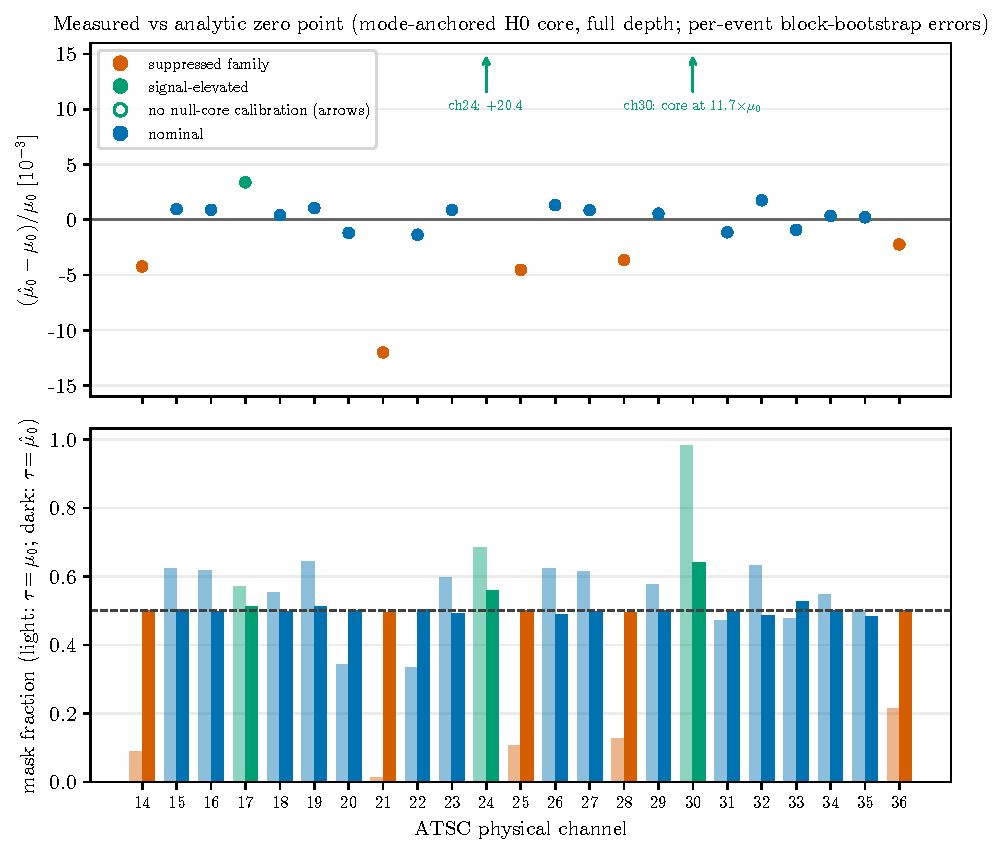
\includegraphics[width=\columnwidth]{fig_empirical_zero_points}
  \caption{Measured vs analytic zero points across the 23 channels: gaps
  in units of $10^{-3}\mu_0$ (top; off-scale channels indicated by
  arrows) and the mask-fraction correction (bottom; light bars: threshold
  at the analytic $\mu_0$, dark bars: at the measured $\hat\mu_0$; dashed
  line: the 0.5 invariant). The suppressed five-channel family and the
  two channels without a null-core calibration are marked with their
  located-mode values (ch24: $+20.4\times10^{-3}$; ch30: mode at
  $11.7\times\mu_0$) --- refusal criteria in
  Section~\ref{sec:zeropoints}.
  Error bars on the gaps are 68 per cent per-event block-bootstrap
  intervals (frames within a capture unit are not independent); they are
  typically smaller than the markers.
  \label{fig:zeropoints}}
\end{figure}

\gpuslot{Phase 1a}{Control certification: full-depth scan of a pilot-free
coarse channel (candidate freq\_ids 637/760/714) through the production
pipeline. Note these controls are pilot-free but still lie \emph{within}
ATSC allocations, so they bound the off-pilot statistic rather than a
DTV-free floor; an out-of-allocation control is therefore
\emph{required}, and the control inventory includes one in the
608--614\,MHz quiet band (freq\_id 484) alongside the in-band
candidates. Fills: control-channel $\hat\mu_0 - \mu_0$ = \gpuval{gap}, mask
fraction = \gpuval{0.45--0.55 acceptance}, and the residual statement
``kept-data excess $\le$ \gpuval{Y}\,dB above the pilot-free floor'' used in
Section~\ref{sec:implications}. A provisional CPU-reference floor from a
bounded raw-file sample (same mathematics as Fig.~\ref{fig:curves}) is in
progress and will be quoted here as provisional if the GPU session is still
unavailable at submission time: \gpuval{provisional gap, n frames, stride}.}

\subsection{Injection--recovery on real baseband (item 3 --- pending)}

\gpuslot{Phase 2}{Injection ladder into real archived baseband at known
SNRs. Fills: linearity figure (recovered vs injected), threshold-crossing
agreement with Fig.~\ref{fig:curves} on real noise, and the per-channel
recovery table.}

\subsection{Radiometer baseline (item 4 --- pending)}

\gpuslot{Phase 2}{Detection-performance comparison on the same injection
ladder at matched false-mask rate, against (i) a total-power radiometer
and (ii) an emulation of the current pipeline's allocation-wide DTV
occupancy rule \citep{chime2025autopower} --- with both detectors'
decisions aggregated to a common cadence, comparing retained clean
exposure and residual contamination under identical injections, not
false-mask rate alone (the 41.94\,ms and visibility cadences are not
directly commensurable). Fills: the sensitivity-advantage headline ---
horizontal gap at $P_{\rm d} = 0.9$ = \gpuval{X}\,dB with CI. If (ii)
proves infeasible, the comparator must be described as a simple
radiometer, not as the flagging status quo.}

\subsection{Cleaning tradeoff (item 5 --- candidate operating point)}
\label{sec:cleaning}

With the zero points calibrated, the remaining freedom is where to put the
mask relative to $\hat\mu_0$. Two results motivate the candidate
operating point (an \emph{exploratory} tradeoff --- the $k<0$ region is
shown in Fig.~\ref{fig:aggr}; a defined contamination metric and the
Phase-2 validation against predetermined criteria are pending):

\textbf{One-sided aggression fails.} Deepening a single ceiling $k\sigma$
below the core keeps exponentially less data while the contamination
\emph{fraction of the kept data rises} (Fig.~\ref{fig:aggr}, colour
vs grey curves): low-tail
excursions --- whatever their origin (Section~\ref{sec:propagation}) ---
concentrate exactly where a deep one-sided keep region selects.

\textbf{The three-arm mask.} The candidate operating point instead
combines
(i) the measured ceiling, masking $F > \hat\mu_0$; (ii) a band floor,
masking $F < \hat\mu_0 - 12\times10^{-3}\mu_0$ against deep differential
fades and reference-side interference; and (iii) a common-mode power veto,
masking frames whose baseband power exceeds a per-capture baseline, which
catches enhancements that lift target and references together and would
otherwise pass the F band. Operationally, each frame's baseband power is
compared against that capture's baseline --- the median power of its
F-core frames, computed \emph{retrospectively} over the capture as an
emulation of a deployment slow tracker --- and common-mode excursions
beyond $5\sigma_P$ are masked even though the power ratio $F$ itself is
blind to them. As evaluated here the baseline is therefore neither
causal nor fully F-independent (its frame selection uses the F core); a
deployed implementation would replace it with a causal running
estimate, whose behaviour Phase 2 characterizes. All three arms' \emph{decisions} are exact fixed-point compares; the
deployed veto's causal tracker (baseline cadence, scatter estimator,
warm-up, and quantization) remains to be specified.
The mean-anchored ceiling also makes the mask self-diagnosing: on any
signal-free channel the mask fraction is expected at $0.5$ under the
validated null model (acceptance window 0.45--0.55) --- a necessary but
not sufficient health check in deployment; it cannot detect every form of
gain drift.

The ceiling's placement \emph{at} the measured core --- rather than
$k\sigma$ above it --- deserves its own defence, because it deliberately
accepts $P_{\rm FA} \approx 0.5$: half of the genuinely clean frames are
sacrificed by construction, capping recovery near 50 per cent before any
transmitter is considered. The loss function is asymmetric by design.
Falsely kept contamination is correlated and does not integrate down;
falsely masked clean frames cost only integration time on the affected
channels. A ceiling at $\hat\mu_0 + 3\sigma$ would keep $\approx 99$ per
cent of clean frames, and Section~\ref{sec:propagation} shows outright
detections ride 8--23 core widths above the band --- but faded pilots
populate a continuum down through the core, so any keep region extending
above the median admits a population of sub-threshold transmitters whose
contamination the floor measurement of Section~\ref{sec:implications}
could no longer constrain from the pilot-free side. Certifiability, not
yield, motivates this candidate operating point; the Phase-2 measurements
test it. Fig.~\ref{fig:aggr} extends to $k<0$ (ceiling above the
measured core); the adopted ceiling sits at $k=0$ exactly (mask
$F>\hat\mu_0$), the boundary of that region. Above the core the kept
fraction tracks the pure-$\mathcal{H}_0$ expectation and the non-null
excess among retained frames stays near zero for the calibrated channels
shown, while any $k>0$ cut both collapses the kept bandwidth and drives
the excess fraction of what remains sharply upward. The operating point is described as \emph{retrospectively motivated}
throughout: the public analysis plan records only the stack-selection
and census-inclusion decisions, and the three-arm thresholds and
ch24/ch30 handling were chosen informally during development (an early
BAO-motivated fixed-threshold approach was considered and abandoned in
favour of the positive-excess rule, with no timestamped record).
\needsdylan{state the predetermined Phase-2 validation criteria the
exploratory operating point will be evaluated against (retention-curve
targets at stated shelf levels).}

\begin{figure}
  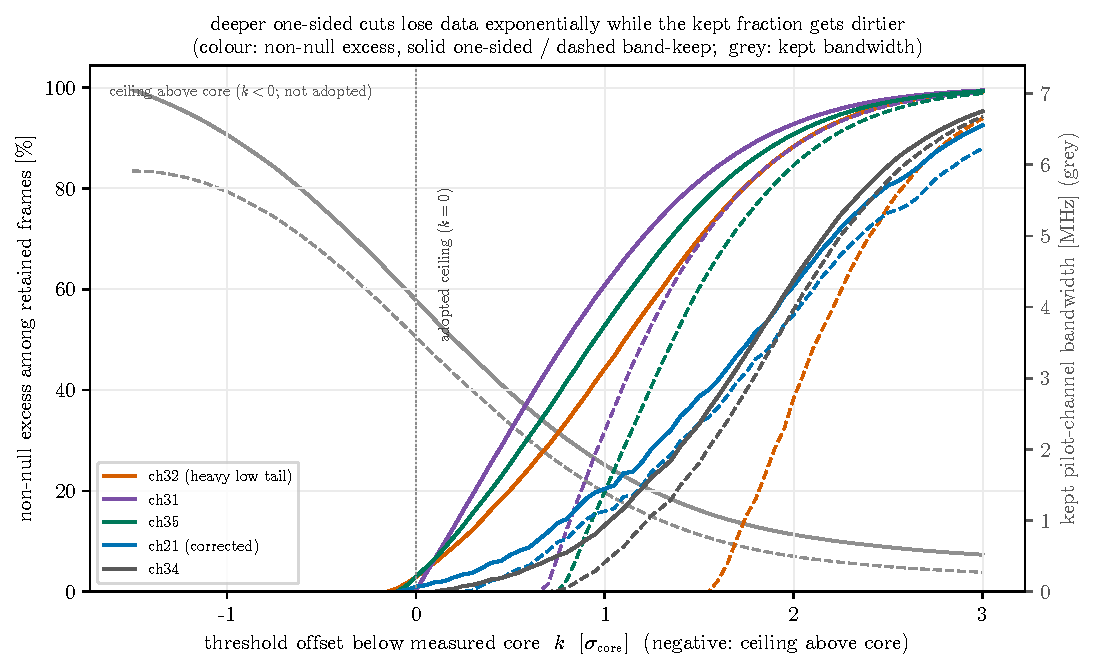
\includegraphics[width=\columnwidth]{fig_aggressive_masking_tradeoff}
  \caption{Why maximum cleaning is not a deeper one-sided cut: as the
  ceiling moves below the measured core ($k>0$), the kept pilot-channel
  bandwidth (grey, right axis) collapses exponentially while the
  non-null excess \emph{among retained frames} (colour, left axis)
  rises --- deeper cuts keep less data and keep it dirtier. The
  deployed rule is the $k=0$ positive-excess ceiling; the $k<0$ region
  (ceiling above core) is shown and not adopted. Colour curves are
  representative channels spanning the tail families (heavy low-tail
  ch31/ch32/ch35, corrected wrap-geometry ch21, nominal ch34; all 23 in
  the supplementary excess figure). The excess is an
  excess-over-model statistic to which instrumental tails, non-Gaussian
  noise, and DTV all contribute, not a DTV-specific contamination
  measure; where signal occupies a large share of a channel's frames it
  is a lower bound.
  \label{fig:aggr}}
\end{figure}

\section{Survey results: 7.6 years of the DTV sky}
\label{sec:survey}

\subsection{Data set}

The production scan processed \textbf{77\,423 of 161\,872} archived
channel--event records (47.8 per cent of the archive; 8\,759 unique
events inventoried, of which 8\,604 appear in the products) across all 23 channels
--- eight channels to 100 per cent of archive depth, the remainder capped
at 2000 events by schedule --- spanning 2018--2026. The per-frame study set
comprises 339\,196 valid frames. Integrated, that is 3.95 channel-hours of
exposure ($\approx 10$ minutes per channel, $\approx 0.18$\,s per sampled
file-event): the survey is snapshot sampling of the DTV sky across
7.6\,yr, not continuous monitoring, and every rate below is a
per-sampled-frame statistic within the stated coverage. A recorded
cross-channel stack (16 channels $\times$ 1548 common events --- 1329
events and 5638 frames after event-keyed alignment --- selected by the
recorded signature-closure search under the amended $\ge$16-channel
rule; Appendix~\ref{app:prereg}) supports the cross-channel analyses;
per-channel results use the full scanned depth.
Table~\ref{tab:perchannel} summarizes.
The archive itself is overwhelmingly \emph{triggered}: of the 161\,872
file-events, 98.2 per cent are FRB/pulsar-triggered baseband captures
and 1.8 per cent scheduled acquisitions; the largest classes are
classified FRB events (42.4 per cent), Crab (B0531+21) commissioning
captures (19.9 per cent), SGR observations (8.1 per cent), and pulsar
backlog/commissioning captures ($\approx$20 per cent combined). The
eight full-depth channels are ch24, ch30, and ch31--36 (their sampled
composition equals the archive composition by construction); the
remaining channels were capped at 2000 events --- 23--38 per cent of
their per-channel archives --- with ch29 extended to 3200 (38 per cent).
For the capped channels the schedule's selection is \emph{not}
class-neutral: on ch14, for example, the 2000 sampled events are 21 per
cent classified-FRB against 44 per cent in that channel's archive, with
commissioning and backlog captures over-represented (per-channel
sampled-vs-archive composition and quarterly exposure are archived as
\texttt{survey\_composition\_by\_channel.csv} and
\texttt{survey\_quarterly\_exposure.csv}). The secular conclusions are
insulated from this bias by the full-depth sampling of the transition
channels and by the classified-FRB stratification of
Section~\ref{sec:secular}; capped-channel rate comparisons across
classes should consult the composition table first.

\begin{table}
  \centering
  \caption{Per-channel survey summary. $\Delta$ = measured zero-point gap
  $(\hat\mu_0-\mu_0)/\mu_0$ in $10^{-3}$; ``clean null core?'' = whether
  a null core was identifiable so that $\hat\mu_0$ is calibrated from it.
  `n' means no usable null core exists (always-dominated ch30;
  signal-elevated ch24 --- physical attributions provisional pending
  census/spectral confirmation), not that the channel's data are suspect.
  Kept fractions of pilot-channel frame-time after the F band (ceiling +
  floor) and after the full three-arm mask. Channels without a null-core
  calibration use the one-sided analytic ceiling and are counted
  uniformly in the measured-retention numbers; the recovery-ineligibility
  rule (Section~\ref{sec:implications}) masks them fully for
  eligibility claims. The ceiling itself has no
  free parameter (the threshold is the null centre); the floor
  ($12\times10^{-3}\mu_0$, five measured core widths) and veto
  ($5\sigma_P$) levels are recorded conventions from the item-5
  tradeoff study, with their exposure costs measured here and their
  cleanliness value pending Phase 2.}
  \label{tab:perchannel}
  \begin{tabular}{rrrcrr}
    \toprule
    ATSC & CHIME & $\Delta$ & null? & kept (F band) & kept (3-arm) \\
    \midrule
    14 & 844 & $-4.2$ & y & 0.486 & 0.456 \\
    15 & 829 & $+1.0$ & y & 0.486 & 0.464 \\
    16 & 813 & $+0.9$ & y & 0.488 & 0.455 \\
    17 & 798 & $+3.4$ & y & 0.194 & 0.152 \\
    18 & 783 & $+0.4$ & y & 0.489 & 0.464 \\
    19 & 767 & $+1.1$ & y & 0.481 & 0.468 \\
    20 & 752 & $-1.2$ & y & 0.488 & 0.470 \\
    21 & 736 & $-12.0$ & y & 0.494 & 0.470 \\
    22 & 721 & $-1.4$ & y & 0.488 & 0.463 \\
    23 & 706 & $+0.9$ & y & 0.482 & 0.454 \\
    24 & 690 & $+20.4$ & n & 0.314 & 0.226 \\
    25 & 675 & $-4.5$ & y & 0.484 & 0.462 \\
    26 & 660 & $+1.3$ & y & 0.466 & 0.425 \\
    27 & 644 & $+0.9$ & y & 0.478 & 0.459 \\
    28 & 629 & $-3.6$ & y & 0.489 & 0.473 \\
    29 & 614 & $+0.6$ & y & 0.486 & 0.470 \\
    30 & 598 & --- & n & 0.017 & 0.015 \\
    31 & 583 & $-1.1$ & y & 0.274 & 0.221 \\
    32 & 568 & $+1.8$ & y & 0.350 & 0.322 \\
    33 & 552 & $-0.9$ & y & 0.418 & 0.385 \\
    34 & 537 & $+0.4$ & y & 0.485 & 0.457 \\
    35 & 521 & $+0.2$ & y & 0.360 & 0.295 \\
    36 & 506 & $-2.2$ & y & 0.491 & 0.465 \\
    \bottomrule
  \end{tabular}
\end{table}

\subsection{The tails are common-mode}
\label{sec:propagation}

Decomposing tail frames shows target and reference powers moving
\emph{together} (on ch32, tail frames sit at 0.35 and 0.38 of the core
baseline in target and references respectively): the excursions are
common-mode power events with a frequency-selective differential across the
12.2\,kHz detector span, not reference-bin artefacts
(Fig.~\ref{fig:taildecomp}). Tail frames cluster in time across channels
($3.5\times$ chance coincidence on ch32, $13\times$ on ch21) --- a
signature environmental events would produce, though correlated
instrumental states (packet loss, gain changes) would cluster as well;
telemetry can test the known instrumental alternatives (below).
Detections sit
far above the mask band: median margins of 19--56$\times 10^{-3}$ above
$\hat\mu_0$ (8--23 core widths), so the $\pm 12\times10^{-3}$ band is not
clipping real detections, and threshold placement at the few-$\sigma$ level
barely moves detection counts.

Common-mode behaviour narrows the field but does not by itself select
propagation: gain steps, packet loss, quantizer-state changes, and
broadband RFI are also common-mode across this 12.2\,kHz span. The low
tail is the sharpest case --- frames at 0.35--0.38 of baseline are power
\emph{deficits}, more naturally missing-sample or gain events than added
emission. \needsdylan{cross-check tail frames against datatrawl/CHIME
telemetry (dropped-packet counts, gain states); reclassify or exclude
instrumentally flagged frames before attributing the remainder to
propagation.}

\begin{figure}
  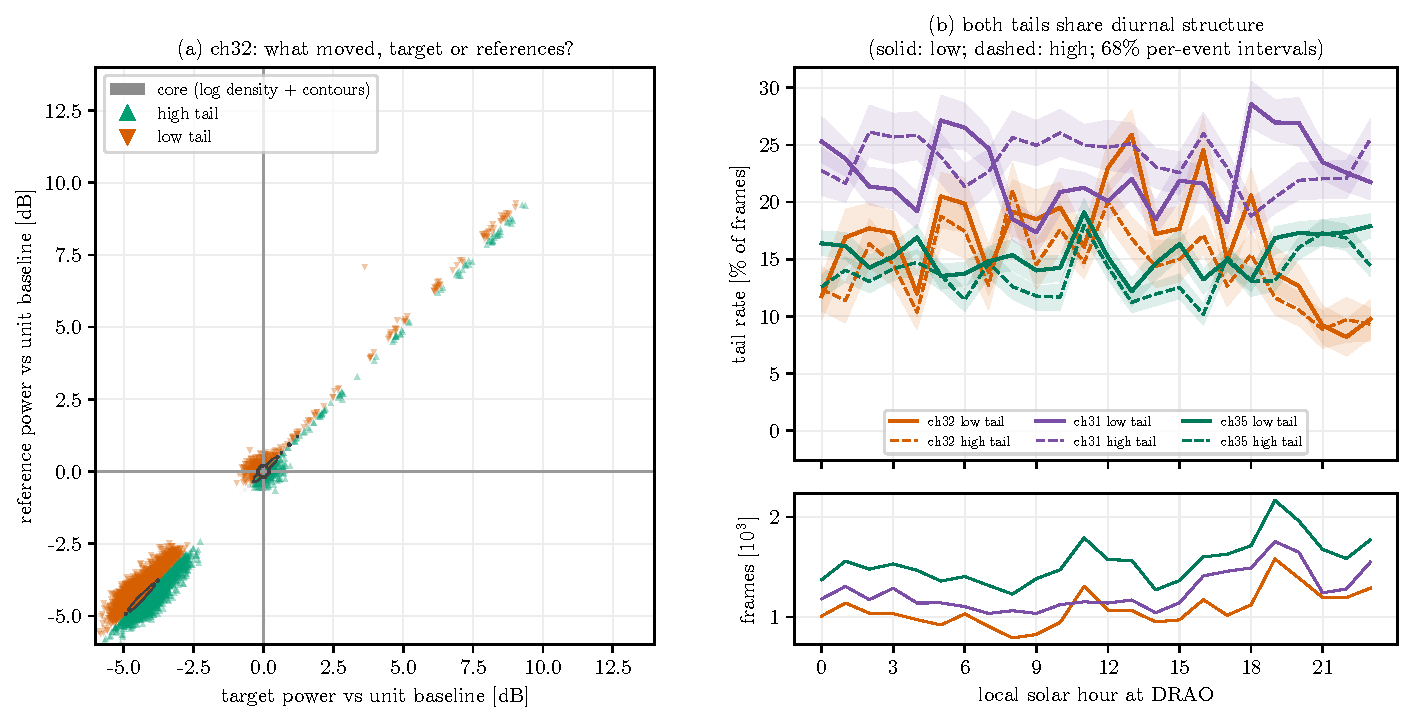
\includegraphics[width=\columnwidth]{fig_tail_decomposition}
  \caption{Tail decomposition. (a) Tail frames ride the target $=$
  reference diagonal (common-mode power change), disfavouring a
  reference-only artefact (it does not exclude all reference
  contamination); the core is rendered as a log-density with contours,
  and core frames share the same diagonal (a common-mode power change
  leaves the ratio $F$ invariant). (b) Low and high tails share diurnal
  structure across channels, with 68 per cent per-event block-bootstrap
  intervals; the lower strip gives the hourly frame denominators.
  Mechanism attribution awaits the telemetry cross-check
  (Section~\ref{sec:propagation}). Channels shown are representatives
  of the heavy-tail family (ch31, ch32, ch35) plus the corrected
  wrap-geometry channel (ch21); the supplementary excess figure gives
  all 23.
  \label{fig:taildecomp}}
\end{figure}

\FloatBarrier  % keep Table 2 / Figs 6-7 from interrupting the 6.3 note
\subsection{Detected-event rates are not stationary}
\label{sec:secular}

The 7.6\,yr time base resolves multi-year rate structure directly
(Fig.~\ref{fig:secular}): ch33's detection rate falls from $\sim$40 to
$\sim$4 per cent by 2020 Q2, consistent with the ATSC spectrum-repack
transition window (completed July 2020; \citealt{fcc2020repack}); ch32's
rate falls from $\sim$35 to $<1$ per cent through 2023 April--May;
ch35's rises from
$\approx 0$ to $\sim$17 per cent in 2021 Q4; ch17's rises from
$\sim$5 (2020) to $\sim$35 per cent (2025), with the capped sampling
leaving no mid-period quarters above the exposure floor, so the
trajectory between those endpoints is unsampled. These are rate
transitions within sampled exposure;
transmitter-side attributions (shutdown, sign-on, repack moves) await
station-level records.

A class-composition robustness check uses the archive inventory join
(Section~\ref{sec:survey}): re-deriving the quarterly rates within the
single largest uniform trigger class (classified FRB events;
capture units assigned to inventory events by day and frame count, 79
per cent of units confidently assigned, ambiguous units excluded), all
four transitions persist with consistent amplitude and timing
(supplementary \texttt{fig\_secular\_frb\_stratum}; 79 per cent of
units confidently assigned --- the unassigned 21 per cent could itself
vary with epoch, so stratified rates remain provisional pending the
archived assignment-quality products): ch33
$0.44/0.39 \rightarrow 0.01$ across the same quarter boundary, ch32
$0.32 \rightarrow 0.03$, ch35 $0.00 \rightarrow 0.17$, and ch17
endpoints $0.03 \rightarrow 0.36$ against $0.05 \rightarrow 0.35$ for
all events. The transitions are therefore not artifacts of the
archive's changing class mix; the three step-transition channels are
additionally sampled at full depth (5118--8304 events), so the depth
cap does not enter them at all. The stratification also exposes one
compositional feature: ch33's apparent 2020 Q4 rebound (rate 0.42) is
carried entirely by non-FRB captures in a small-exposure quarter (66
valid frames) and is absent from the FRB stratum. \needsdylan{corroborate each transition against FCC/ISED station
records before any causal wording returns. Partial web verification
(2026-07-17): CBUT-DT's repack move to RF~35 is confirmed as 2020-05-01
(88.5\,kW, Mount Seymour) --- 18 months before the observed ch35
onset, so the interim-vs-full-facility question stands (ISED);
KDYS-LD (ch32's strongest census entry) is still listed on RF~32 in
current market listings with no visible 2023 event in reachable public
sources, which \emph{weakens} the KDYS-LD attribution for the 2023
April--May fall unless its FCC application history (LMS, not publicly
reachable here) shows a silent period or facility change; ch33
(Okanagan relay history) and ch17 (K17KR-D, CIVI-2) remain unresolved
pending ISED/LMS lookups.}

The episodic set itself is defined by a \emph{full-period} tail
fraction (Fig.~\ref{fig:secular}), a criterion that dilutes any loud
epoch short relative to a channel's total exposure. A completeness
scan --- the same quarterly re-derivation extended to every calibrated
channel in both strata (archived as
\texttt{survey\_quarterly\_rates\_all23.csv}) --- finds exactly one
further multi-year transition hiding below that criterion: ch34 runs
at 3--8 per cent from 2018 through 2020, steps down to $\approx$2 per
cent through 2021, and fluctuates about 1 per cent thereafter
(full-depth sampling; the step persists in the FRB stratum), its
full-period tail diluted to 2.3 per cent by the long quiet majority.
One capped channel adds a sampled loud interval rather than a resolved
transition: ch27 reads 38 per cent in 2020 Q3 (37 per cent in the FRB
stratum) against $\le$1.3 per cent in every 2025--26 quarter, with the
interior unsampled under the depth cap. Beyond these two, no channel
outside the episodic set sustains a rate above 3 per cent for
consecutive quarters. Both epoch effects carry into the channel
ordering of Section~\ref{sec:implications}.

The
aggregate episodic-channel detection rate swings from $\sim$25 per cent
(2019--2020) to $\sim$11 per cent (2022--2024). After removing this secular
drift year-by-year, the residual seasonal modulation is only
$1.24\times$ peak-to-trough and not coherent across channels
(Fig.~\ref{fig:seasonal}, Appendix~\ref{app:diagnostics}):
secular rate change dominates; climatology is second order at this
sensitivity.

The deployment lesson is structural: sampled rates changed substantially
between epochs separated by order-year intervals,
\emph{in both directions} (a channel with low sampled rates until 2021
now shows among the highest; the Q3-2023 rate collapse left a blacklisted
channel with a low sampled rate). Continuous per-frame detection against
a measured zero point tracks such changes at frame cadence ---
complementing the dynamic allocation-wide occupancy rule the current
CHIME pipeline already applies at visibility cadence
\citep[Appendix~A]{chime2025autopower} --- and the mask-fraction health
check is designed to flag gross calibration drift.

\begin{figure}
  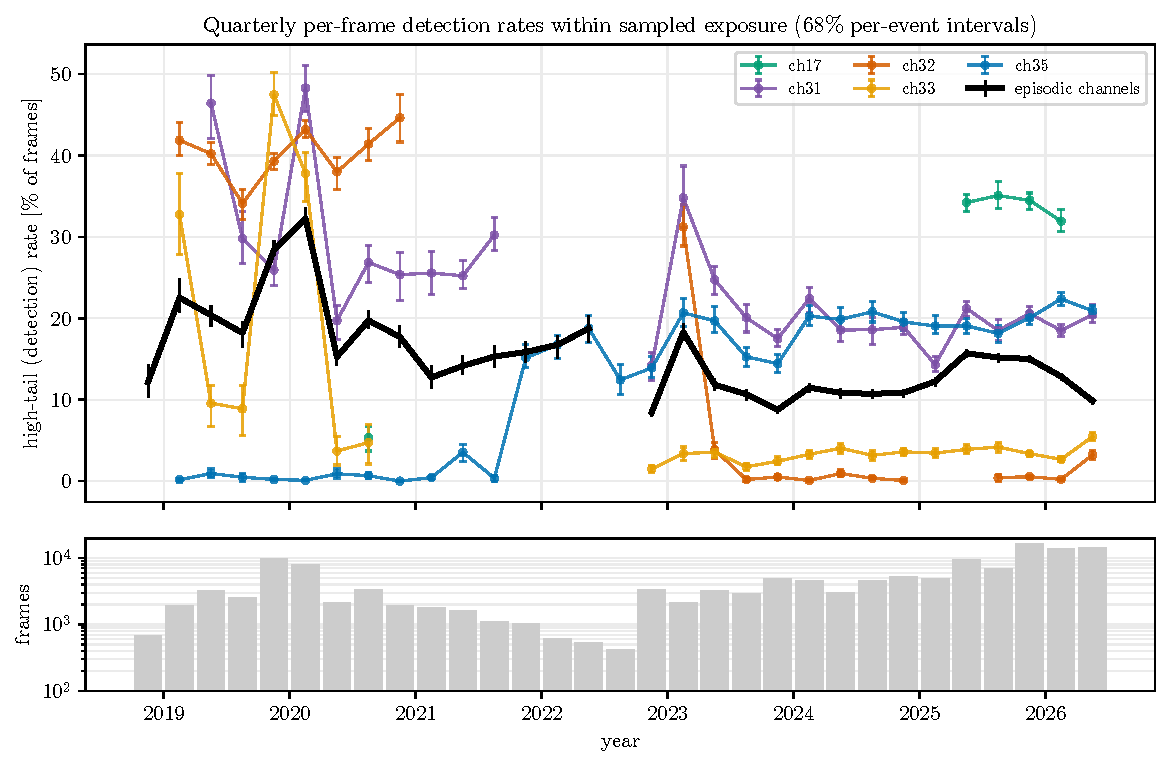
\includegraphics[width=\columnwidth]{fig_secular_rates}
  \caption{Quarterly per-frame detection rates within sampled exposure,
  2018--2026: the 2020 repack-consistent collapse (ch33), a 2023 rate
  collapse (ch32), a 2021 rate onset (ch35), and a five-year rise (ch17).
  Sampled rates changed substantially between epochs separated by
  order-year intervals, in both directions. Lines break across quarters
  without sampled exposure ($\le 200$ frames per channel; $\le 500$ for
  the aggregate); points carry 68 per cent per-event block-bootstrap
  intervals; the lower strip shows sampled frames per quarter. The episodic
  set is defined quantitatively: calibrated channels with high-tail
  fraction $>3$ per cent (channels 17, 26, 31, 32, 33, 35). The five
  with resolved multi-year transitions are drawn; ch26 (high-tail 4.0
  per cent, just over threshold) is omitted for legibility, channels
  outside the set sit near 1 per cent in sampled quarters --- apart
  from two sub-criterion epoch effects (ch27, ch34) established in the
  text --- and the black aggregate spans all
  six.
  \needsdylan{confirm the channel--transmitter identifications
  (FCC/ISED corroboration).}
  \label{fig:secular}}
\end{figure}

\FloatBarrier  % keep Fig. 7 from splitting the section-opening sentence
\section{The operating point and eligible exposure}
\label{sec:operating}

Evaluated at full scanned depth, the ladder of pilot-channel frame-time
kept by the three-arm mask --- expressed as equivalent bandwidth on the 23
pilot-bearing channels --- is
\begin{center}
\begin{tabular}{lr}
  \toprule
  rule & kept of 8.984\,MHz \\
  \midrule
  analytic ceiling ($F \le \mu_0$) & 4.708\,MHz \\
  measured ceiling ($F \le \hat\mu_0$) & 4.230\,MHz \\
  $+$ band floor & 3.784\,MHz \\
  $+$ common-mode power veto & \textbf{3.512\,MHz} \\
  \bottomrule
\end{tabular}
\end{center}
The final rung, \textbf{3.512\,MHz} (39.1 per cent), is the rule's
\emph{measured retention}: the two channels without a null-core
calibration run the same rule at the analytic constant and are counted
uniformly. For \emph{eligibility} claims the recovery-ineligibility
rule of Section~\ref{sec:implications} masks those two channels fully
--- retained frames there carry no cleanliness certification until the
Phase-2 measurements --- giving \textbf{3.418\,MHz} (38.0 per cent)
deployment-eligible, the figure carried into the eligibility
projections. The first step
of the ladder is a calibration correction, not a cut; each further arm
changes the retained set in the intended direction, with its cleanliness
value to be established by the floor measurement and Phase-2 tests. The veto's thresholds are strikingly thin ---
the per-frame power scatter on quiet channels is only 0.04--0.06 per cent
(frame sums average $\sim 2^{25}$ samples), so a $5\sigma_P$ veto sits just
$+0.01$\,dB above baseline yet costs only 3--7 per cent of band-kept frames
there (18--28 per cent on propagation-active channels). Its effect on the
kept data is decisive: the 99.9th-percentile power excess of frames the F
band alone would keep is $+2.4$ to $+9.8$\,dB depending on channel; after
the veto it collapses to $\approx +0.01$\,dB on quiet channels
(Fig.~\ref{fig:veto}) --- by construction, since the veto threshold sits
there: the clipped tail shows the veto doing its job. The independent
evidence for the ``cleanest kept data'' objective is the Phase-1a floor
measurement, not this tail.

These are pilot-channel quantities; the deployment semantics of
Section~\ref{sec:whyframes} scale them into \emph{equivalent
allocation-time made eligible by the mask} --- eligible, not recovered,
because the current pipeline's masks may already retain part of it and
downstream masks may reject part of what this mask keeps. On the
archive-weighted sampling, the Table~\ref{tab:perchannel} keep fractions
project to $\approx 52.5$\,MHz under the recovery-ineligibility rule
(ch24 and ch30 fully masked; 38.0 per cent deployment-eligible) --- the
figure carried forward --- with $0.391 \times 138 \approx 53.9$\,MHz
as the rule's raw measured retention counted uniformly over all 23
channels.
Both are preliminary eligibility projections, quoted before exact
coarse-channel boundary accounting at allocation edges and before a
simultaneity-controlled recompute on the common stack.
\needsdylan{recompute on the recorded common stack; once the
calibration-refused default is confirmed, carry only the excluded-channel
number forward. A representative allocation-wide spectrogram plus one
quantitative full-band test suffices for this paper; the full-archive
mask-expansion run is out of scope.}

\begin{figure}
  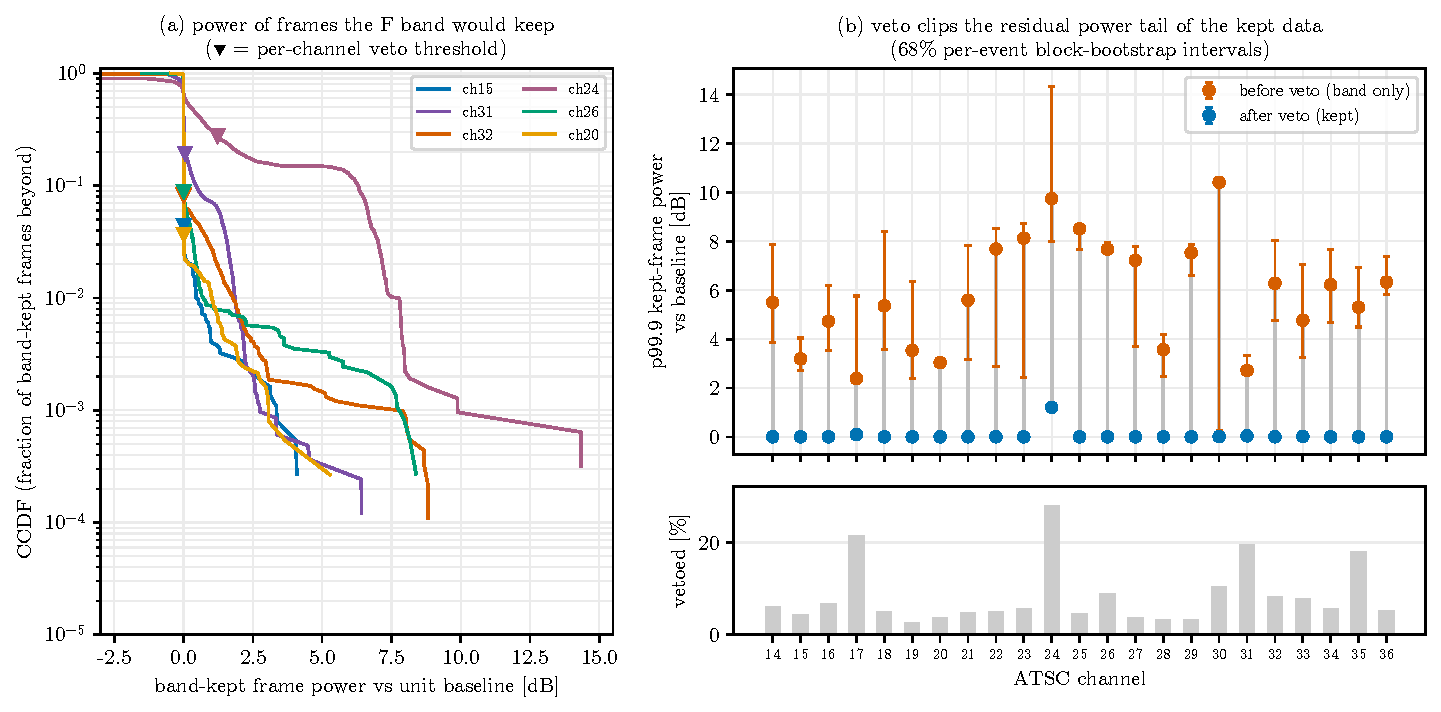
\includegraphics[width=\columnwidth]{fig_threearm_veto}
  \caption{The common-mode power veto: (a) power CCDFs of band-kept
  frames with per-channel $5\sigma_P$ thresholds, for six channels
  spanning the observed classes --- quiet cores (ch15, ch20, ch26), heavy
  episodic tails (ch31, ch32), and one calibration-refused channel
  (ch24); (b) the p99.9 kept-data power tail before/after the veto with
  68 per cent per-event block-bootstrap intervals, and the vetoed
  fraction per channel in the lower strip.
  \label{fig:veto}}
\end{figure}

\FloatBarrier
\section{Implications for 21\,cm cosmology and deployment}
\label{sec:implications}

\subsection{What the eligible exposure would buy}

The mask's measured retention is 39.1 per cent of pilot-channel
frame-time (3.512 of 8.984\,MHz); under the recovery-ineligibility rule
the deployment-eligible fraction is 38.0 per cent, making $\approx
52.5$\,MHz of
allocation-time \emph{eligible} under allocation-wide gating
(Sections~\ref{sec:whyframes} and \ref{sec:operating}), in the band that
carries the high-redshift half of the CHIME BAO range
($1.34 < z < 2.02$). Because correlated RFI
residuals do not integrate down, the value of eligible exposure is
conditional on its cleanliness; the candidate operating point above was
chosen with exactly that objective --- its achieved cleanliness remains
to be established --- and the floor measurement --- kept-data excess
$\le$ \gpuval{Y}\,dB above the control-channel pilot-free floor (Runbook
Phase 1a; Section~\ref{sec:zeropoints} notes the controls' in-allocation
limitation) --- is the central number this paper awaits. Combined with the
retention-probability calibration of Section~\ref{sec:shelfconv}
(Phase 2) --- and only once the out-of-allocation control and the
wideband occupancy/decorrelation model of Section~\ref{sec:shelfconv}
exist --- it would constrain, probabilistically, the shelf a
sub-threshold pilot could hide across its allocation. With those in
hand, eligible channels would carry a quantified residual budget
relative to the thermal floor.

Because BAO-grade data ultimately admits only the highest-confidence
exposure, the 23 channels are not interchangeable, and the measured
properties of this paper already order them. The
strongest candidates for first adoption are the eight quiet
nominal-geometry channels --- 15, 16, 18, 19, 23, 27, 29, and 34 ---
with zero points within $1.1\times10^{-3}$ of analytic, core occupancy
near 90 per cent, and no cell anomalies: roughly 3.1\,MHz of
pilot-band at $\approx$50 per cent kept. Six of the eight show
detection rates at the 1--2 per cent level with no sustained excursion
in any sampled quarter; the completeness scan of
Section~\ref{sec:secular} qualifies the other two by epoch. ch34's
step is measured at full depth --- 3--8 per cent through 2020,
$\approx$2 per cent in 2021, $\approx$1 per cent after --- so its
first-adoption standing applies to exposure from 2021 onward. ch27's
record is endpoints-only under the depth cap (38 per cent in 2020 Q3,
$\le$1.3 per cent in every 2025--26 quarter): its certified-quiet
standing rests on the 2025--26 coverage, and the unsampled 2021--2024
interior remains uncertified either way until the full-archive
extension completes. Earlier archival data on both inherits the
per-epoch treatment of the episodic set below. Channels 20 and 22 sit one notch behind the eight on a
single axis: equally quiet (flat near 1 per cent) and equally occupied
($\ge$92 per cent core occupancy), but with small, statistically
significant static shifts ($-1.2$ and $-1.4\times10^{-3}$, formally
$\sim$40$\sigma$) that no geometric mechanism accounts for, so their
calibrations rest on the measured table alone rather than on its
agreement with the analytic anchor. Behind them, in decreasing
confidence: the geometric family (14, 21, 25, 28, 36), whose
calibrations are empirical corrections without a working mechanistic
model and therefore lean on the re-measurement cadence and health
check to catch drift (ch14 additionally hosts the most crowded target
cell in the band, three co-channel carriers); the episodic set (26,
31, 32, 35), whose contamination and exposure are epoch-dependent, so
per-epoch eligibility should consult the archived quarterly tables;
ch17, the weakest trusted calibration (19.5 per cent occupancy against
the 15 per cent floor) with a rising multi-year detection rate and a
plausible trajectory into refusal at a future re-measurement; and
ch33, which every per-frame diagnostic scores as clean precisely
because the detector's response to its measured occupant is suppressed
by $-17$\,dB --- its kept frames should be treated as uncertified
until the epoch-split accumulation of
Appendix~\ref{app:diagnostics} resolves whether the guard carrier is
current. The refused pair (24, 30) closes the list under the
recovery-ineligibility rule. One caveat is universal rather than
per-channel: signal below the width-crossing scale retains at
$\approx$0.5 on \emph{every} channel by construction, so the ordering
above ranks presence probability, blindness, and calibration
confidence --- not immunity.

The ordering translates directly into survey terms through
$z = \nu_{21}/\nu - 1$ ($\nu_{21} = 1420.4$\,MHz). The contaminated
band spans $1.336 < z < 2.022$, bounded above in frequency by the
protected radio-astronomy allocation at 608--614\,MHz --- the only
DTV-free slot in the range. The
first-adoption eight would gate exposure in eight 6-MHz allocations
distributed across nearly that entire interval --- from ch34 at
$z = 1.383$--$1.407$ to ch15 at $z = 1.947$--$1.984$, a summed
$\Delta z \approx 0.25$ of the 0.69 available --- rather than
clustering at either end (eligibility here is frame-time on these
allocations, roughly half of it kept, not additional bandwidth), and
channels 20 and 22 would add two interior slices ($z =
1.774$--$1.807$ and $1.711$--$1.742$). Conversely, every channel this
construction cannot yet certify subtracts a narrow notch rather than
a redshift interval: the refused pair removes $z = 1.650$--$1.680$
(ch24) and $1.483$--$1.510$ (ch30), and ch33's blind spot spans
$1.407$--$1.432$ --- each $\Delta z \approx 0.02$--$0.03$. The
conservative tiering therefore costs depth on individual slices ---
kept frame-time on less-trusted channels --- but not reach: no
contiguous redshift range within the DTV band is forfeited wholesale.

The design is intended to reduce selection
coupling: the detector's own selection acts on a statistic diluted
$\sim$1/128 relative to any one fine bin (though dilution of the
statistic does not by itself dilute the science-band transfer), and the
veto arm's compare uses baseband power rather than $F$, though as
evaluated here its baseline frames are selected using the $F$ core
(Section~\ref{sec:operating}), so it is not fully F-independent; a
deployed causal tracker would restore independence. Its
magnitude will be quantified in Phase 2. What this paper deliberately
does \emph{not} claim is end-to-end cosmological safety: that standard ---
forward-modelling the mask through signal and noise simulations, with the
mask's correlation against Earth-rotation angle monitored explicitly ---
is set by the current auto-power analysis \citep{chime2025autopower}, and
meeting it on eligible DTV exposure belongs to a future CHIME
pipeline/overview update, not to this paper.

\subsection{Deployment path}

Deployment of the F-band arms is a constants swap in an integer compare
the kernel already evaluates: the candidate operating point's measured
constants replace (tns,
rnss) with the per-channel rational pairs of Appendix~\ref{app:constants},
which are built in the kernel's own half-threshold convention and load
into the existing checked rational entry point unchanged. We record the
integration status plainly: that entry point has been exercised --- and
CPU/GPU parity proven, with a zero rational-overflow count --- with
testbench constants only; no kernel run has yet been handed the
measured pairs, and the band floor is the same compare with the
opposite sense, which does not yet exist as a kernel entry point. The
remaining components are new, if small: the floor-sense compare, the veto
arm's u64 power compare with a causal slow-tracked threshold, the
allocation-wide broadcast of each pilot channel's decision
(Section~\ref{sec:whyframes}), time alignment with downstream products,
and the documented default when calibration is unavailable or refused:
a channel whose null-core calibration refuses (the estimator's trust
flags fire because no measurable pilot-free population exists) is
declared \emph{recovery-ineligible} --- the detector still runs and
masks there, but its output does not gate recovery, and the channel
remains fully masked. By construction this class is a small minority
arising only in unavoidable cases --- here 2 of 23 channels, each
hosting a persistent transmitter that leaves the sky with no quiet
frames --- and its membership is re-evaluated whenever the zero-point
table is re-measured.
On acceptance: no scalar acceptance pair (a maximum tolerable kept
shelf level and a false-retention probability at it) is adopted,
deliberately --- the deployed rule has no free threshold to engineer
toward such a requirement, and Section~\ref{sec:shelfconv} shows a
per-frame pair would not bound retained contamination without an
occupancy model. The acceptance interface is instead the measured
retention curve $P(\mathrm{retained} \mid \rho_{\rm shelf})$ from
the Phase-2 injection ladder: a downstream analysis states its own
tolerable shelf level and reads the achieved false-retention
probability off the curve. Kotekan integration, throughput, and latency measurements
accompany the GPU runs; full commissioning belongs to a future CHIME
pipeline/overview update. Annual re-measurement of the
zero-point table is cheap, and the mask-fraction $\approx 0.5$ health
check is designed to flag gross drift without auxiliary calibration (its
false-alarm and latency behaviour is part of the Phase-1 verification).
We record, without implementing, the natural automation: the kernel's
exact per-frame integer readback supports continuous per-channel
accumulation of the $F$ histogram, so the re-measurement could run as
a per-channel slow loop --- the same estimator and trust flags on a
rolling window, with atomic constant swaps --- rather than as a
periodic campaign; it is deliberately deferred, and no cross-channel
information would enter at any point. The construction should
adapt to other broadcast standards that provide deterministic pilots or
continual reference structure (ATSC~3.0, DVB-T, ISDB-T), though each
requires its own weight bank and validation --- a possible future
extension, not a demonstrated result of this paper.

\section{Conclusions}
\label{sec:conclusions}

We have built and characterized a per-frame DTV detector for CHIME keyed
to the ATSC pilot: three int4 matched filters and one integer compare,
exact in the correlator's native arithmetic, with rational thresholds
recorded verbatim in every product. Synthetic validation against a
bit-exact CPU reference lies within $\approx$0.5\,dB of ideal detection
statistics at the audited per-trial dimensionality, with capture loss
matching the $\mathrm{sinc}^2$ prediction; deployment-scale regeneration
of the curves is pending (Section~\ref{sec:synthetic}). On-sky calibration across 339\,196 frames
measures the null-core zero point of every channel that admits one (21 of
23) to parts in $10^{3}$ --- consistent with the ideal
independent-row core width --- resolves a five-channel family of static
offsets associated with reference-bin geometry, falsifies the natural
PFB-based alternative, and refuses to fit the two channels where no clean
core exists. In the sampled record, detection rates are non-stationary in
both directions, separated by order-year intervals --- the structural
argument for continuous detection over any static list.
The retrospectively motivated candidate operating point measures 39.1
per cent retention of pilot-channel frame-time on the sampled archive,
of which 38.0 per cent is deployment-eligible under the documented
recovery-ineligibility rule (the two calibration-refused channels stay
fully masked), with the kept power tail
clipped at the veto threshold by construction --- achieved cleanliness
pending Phases 1--2.
Allocation-wide, this makes a preliminary $\approx$52.5\,MHz of exposure
eligible for recovery, pending the simultaneity-controlled accounting,
the allocation-boundary accounting, and the representative full-band
expansion test of Section~\ref{sec:operating}.

What remains is measurement, comparison, and integration: the
deployment-scale regeneration of the detection curves, the
control-channel scan (Runbook Phase 1a; the CPU/GPU parity check is
now measured in Section~\ref{sec:synthetic}), the
real-baseband injection ladder with its retention-probability
calibration, a common-cadence comparison against the current pipeline's
DTV rule --- retained clean exposure and residual contamination under
identical injections (Phase 2) --- held-out re-evaluation of the
calibration,
and --- for a future CHIME pipeline/overview update --- downstream
validation to the forward-modelled standard of
\citet{chime2025autopower}. The F-band arms deploy as a per-channel
constants swap; the veto, broadcast, and alignment components are small
but new. The construction should adapt wherever a broadcast standard
provides a deterministic pilot or continual reference structure, as
future work.

\section*{Acknowledgements}
D.J.G. and K.B. are members of the CHIME Collaboration. D.J.G. and K.B.
acknowledge the Directorate for Mathematical and Physical Sciences,
Division of Astronomical Sciences, NSF Award No.~2307581. FRB research
at WVU is supported by NSF grants 2006548 and 2018490.

We acknowledge that CHIME is built on the traditional, ancestral, and
unceded territory of the Syilx Okanagan people. We are grateful to the
staff of the Dominion Radio Astrophysical Observatory, which is operated
by the National Research Council of Canada. CHIME operations are funded
by a grant from the NSERC Alliance Program and by support from McGill
University, the University of British Columbia, and the University of
Toronto. CHIME was funded by a grant from the Canada Foundation for
Innovation (CFI) 2012 Leading Edge Fund (Project 31170) and by
contributions from the provinces of British Columbia, Qu\'ebec, and
Ontario. The CHIME/FRB Project --- whose triggered baseband captures
constitute the archive analysed in this work --- was funded by a grant
from the CFI 2015 Innovation Fund (Project 33213) and by contributions
from the provinces of British Columbia and Qu\'ebec, and by the Dunlap
Institute for Astronomy and Astrophysics at the University of Toronto.
Additional support was provided by the Canadian Institute for Advanced
Research (CIFAR), the Trottier Space Institute at McGill University, and
the University of British Columbia. The CHIME/FRB baseband recording
system is funded in part by a CFI John R.\ Evans Leaders Fund award.

This research used the facilities of the Canadian Astronomy Data Centre
(CADC), operated by the National Research Council of Canada with the
support of the Canadian Space Agency, and the Canadian Advanced Network
for Astronomical Research (CANFAR). The Green Bank Observatory, whose
data supported development of this work's tooling, is a facility of the
National Science Foundation operated under a cooperative agreement by
Associated Universities, Inc. The National Radio Astronomy Observatory
is a facility of the National Science Foundation operated under
cooperative agreement by Associated Universities, Inc.
\needsdylan{confirm member-paper requirements per current CHIME
publication policy (collaboration text, author-list handling) and the
exact current CADC/CANFAR standard lines.}

\section*{Data Availability}
\label{sec:availability}

\textit{pilot-proxy} and \textit{datatrawl} are open source
(\texttt{github.com/\allowbreak WVURAIL/\allowbreak pilot-proxy},
\texttt{github.com/\allowbreak WVURAIL/\allowbreak datatrawl}); tagged
releases with Zenodo DOIs
will accompany submission, including the detector data sheet and user
guide, cited as software per Force11/RASTI policy. The repository's
\texttt{analysis/} directory regenerates every figure and table in this
paper deterministically from the small archived per-frame products
(byte-identical CSV regeneration is part of its test;
Appendix~\ref{app:repro}); CHIME baseband data are available through CADC
per CHIME data policy. Derived per-frame products, the measured zero-point
and threshold constants tables, and the sweep summaries are archived with
the paper.


\bibliographystyle{plainnat}
\bibliography{refs}

\appendix
% Appendices -- input AFTER \bibliography in both wrappers (journal order).
\FloatBarrier  % keep appendix floats out of the reference list

\section{All-channel diagnostics}
\label{app:diagnostics}
Full coarse-channel and pilot-zoom integrated spectra for all 23
channels (raw, instrument-removed, and after-analytic-mask variants at
shared
per-channel scales, with the detector's target, skipped-guard, and
reference cells marked) and the per-channel F distributions about the
operating threshold (kept/masked split, both zero points, tail bounds,
and the sub-threshold leak estimate in a single view) are provided as
supplementary figures (\texttt{fig\_spectra\_all23\_*},
\texttt{fig\_excess\_threshold\_all23}), together with the diurnal
mask-fraction diagnostic. \needsdylan{decide: formal RASTI supplementary
material vs.\ repository-only, and update this sentence accordingly.}

Across all 23 channels the pilot-zoom panels validate the cell
geometry on-sky: extracted carriers isolate in the target cell,
sidelobe structure confines to the skipped guards, and no persistent
narrow line above the extraction threshold is apparent in the
reference cells. Resolved against the cells, 18 of the 19 line-bearing
channels place their dominant extracted line inside the target cell,
typically within a few hundred Hz of nominal; ch24's secondary lines
sit at $+522$\,Hz (in-cell) and $+3121$\,Hz (skipped guard, where the
target term recovers $-32$\,dB). The exception is ch33, whose
\emph{only} extracted lines sit in the lower skipped guard ($-3.6$\,kHz
at 21\,dB integrated SNR and $-2.8$\,kHz at 13\,dB; target-term
recovery $-17$ and $-23$\,dB): a carrier parked there is strongly
attenuated, not invisible, but the detector's response to it is
suppressed by more than an order of magnitude. This is the
operationally hazardous class
--- a persistent co-channel station on the nominal pilot is detected
and masked most of the time (analytic-mask fractions 0.69 on ch24 and
0.98 on ch30), costing exposure only, whereas
an off-nominal pilot is DTV the mask responds to only weakly, and its
symbol shelf would ride into kept data largely undetected (to be
bounded by the pending Phase-1a pilot-free floor measurement).
Licensing is consistent with, but does not establish, the hazard: the
census \emph{source} carries no frequency-tolerance entry for
translator/LPTV classes (a blank field, not evidence that regulatory
tolerances are absent), and ch33's current occupant is a translator. Because the
accumulation is full-depth, the guard carrier could equally be the
integrated signature of the departed pre-repack occupant; an
epoch-split accumulation would distinguish the two. Re-centring ch33's
target weight onto the measured offset is possible in principle --- a
per-channel constants change within the existing machinery --- but is
deliberately not implemented; we record the option for operations.
An automated line search over the before-mask spectra (running-median
background, 23.84\,Hz bins) outside a $\pm$10\,kHz exclusion around the
nominal pilot (covering the $\pm$7.63\,kHz detector-cell support plus a
buffer) and $\pm$100\,Hz around the coarse-channel DC finds six narrow
lines above 4\,dB of local background across the 23 coarse channels
(Table~\ref{tab:spurs}). Five lie within 9.5\,Hz --- less than half a
spectral bin --- of rational fractions of the coarse sample rate
$f_{\rm s}=390.625$\,kHz in baseband ($\pm f_{\rm s}/5$,
$\pm f_{\rm s}/3$, $\pm 2f_{\rm s}/5$), each in a single coarse
channel, and their prominence over the local background is unchanged
under the analytic mask: consistent with instrumental or
digital-processing spurs, pending operations confirmation. The ch17
line is unidentified and retained. The nearest line lies more than
73\,kHz from detector-cell support (75\,kHz from the nearest cell
centre), 24 fine bins away, so none can materially perturb the
statistic; they remain ordinary narrow-band RFI for downstream
flagging. Notches are applied only to the supplementary plotting
copies; every detector and mask result in this paper uses unnotched
data. ``After mask'' in these supplementary spectra denotes the
original analytic positive-excess production mask recorded in the
archived products (mean masked fraction 0.476, matching the 4.708\,MHz
analytic-ceiling rung of the ladder in Section~\ref{sec:operating}),
not the candidate three-arm rule
(inventory archived as \texttt{instrument\_tones.csv}).
\needsdylan{optional: confirm spur provenance (clock fractions in the
per-channel digitizer/processing chain) with CHIME operations.}

\begin{table}[b]
  \centering
  \caption{Narrow lines above 4\,dB of local background found by the
  automated search (before-mask integrated spectra, 23.84\,Hz bins;
  search domain as stated in the text). This is the complete inventory
  over all 23 coarse channels, not a selection. Prominence (dB) is measured
  against each spectrum's own local running-median background;
  $\Delta$ is the change in that \emph{prominence} under the analytic
  positive-excess mask --- not an absolute-amplitude change, and no
  invariance under the veto or the full three-arm rule is claimed.
  ``Notched'' lines, and the coarse-channel DC spur in every channel,
  are replaced by the local background in the instrument-removed
  supplementary plotting copies only.}
  \label{tab:spurs}
  \begin{tabular}{rrrrrl}
    \hline
    ch & $f_{\rm bb}$ [kHz] & dB & \# bins & $\Delta$ [dB] &
    identification \\
    \hline
    14 & $-78.130$  & 16.4 & 2 & $+0.1$ & $-f_{\rm s}/5$ (notched) \\
    17 & $+157.285$ & 6.1  & 1 & $0.0$  & unidentified (retained) \\
    25 & $-130.200$ & 6.1  & 1 & $0.0$  & $-f_{\rm s}/3$ (notched) \\
    28 & $+130.200$ & 8.8  & 2 & $+0.1$ & $+f_{\rm s}/3$ (notched) \\
    29 & $+156.260$ & 18.6 & 7 & $0.0$  & $+2f_{\rm s}/5$ (notched) \\
    34 & $-156.260$ & 12.6 & 3 & $-0.3$ & $-2f_{\rm s}/5$ (notched) \\
    \hline
  \end{tabular}
\end{table}
Two of the diagnostics carry claims made in the main text and are
reproduced here: the falsified PFB-prototype prediction
(Fig.~\ref{fig:pfbpred}; Section~\ref{sec:zeropoints}) and the residual
seasonal modulation after secular detrending (Fig.~\ref{fig:seasonal};
Section~\ref{sec:secular}).

\begin{figure}[t]
  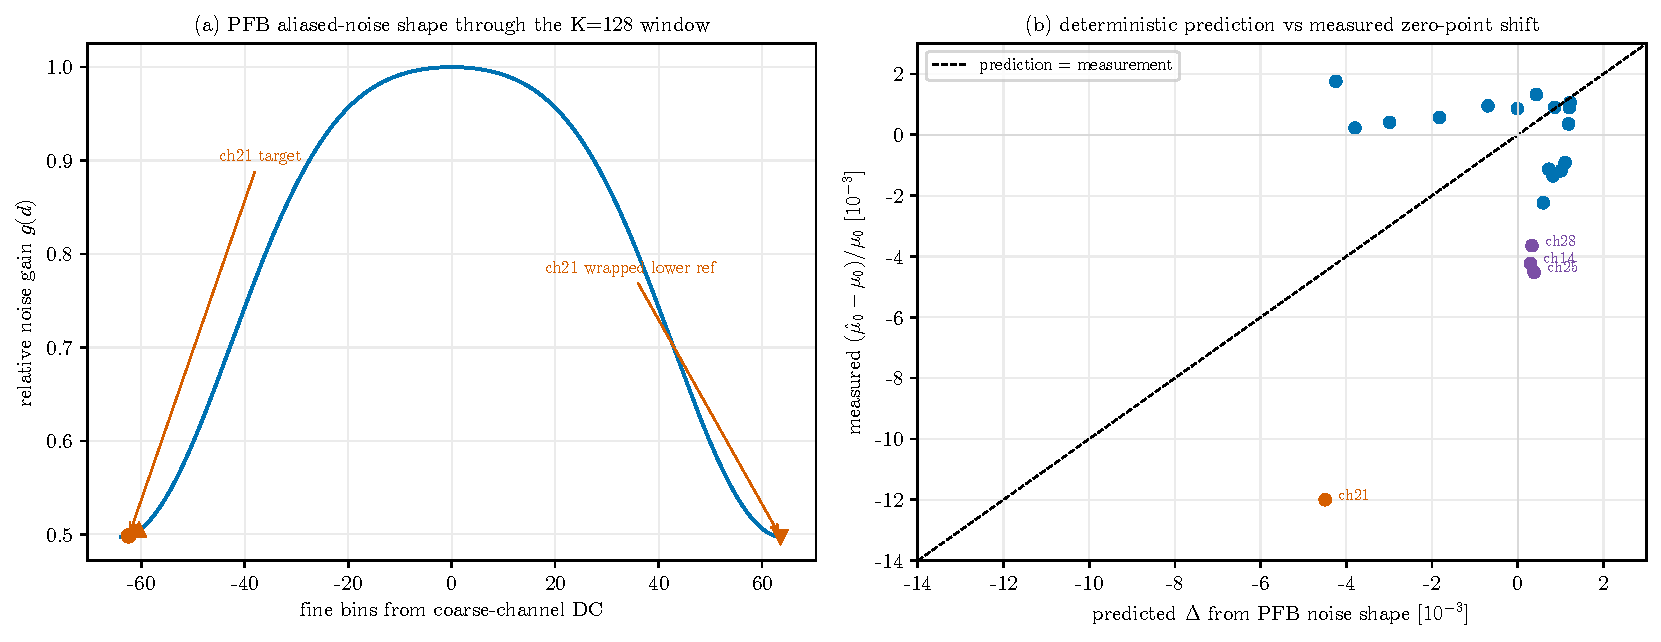
\includegraphics[width=\columnwidth]{fig_pfb_zero_point_prediction}
  \caption{The falsified physics-based alternative --- a model test,
  not a per-channel quality ranking. (a) Aliased-noise
  gain of the 4-tap sinc-Hamming reference PFB prototype through the
  $K=128$ window, with ch21's target and wrapped lower-reference
  placements marked. (b) Predicted vs measured zero-point shifts (dashed:
  prediction $=$ measurement): the prediction fails on the near-edge
  channels 18/29/32/35, where measurements are consistent with zero, and
  captures only a third of ch21's shift
  (Section~\ref{sec:zeropoints}).
  \label{fig:pfbpred}}
\end{figure}

\begin{figure}[t]
  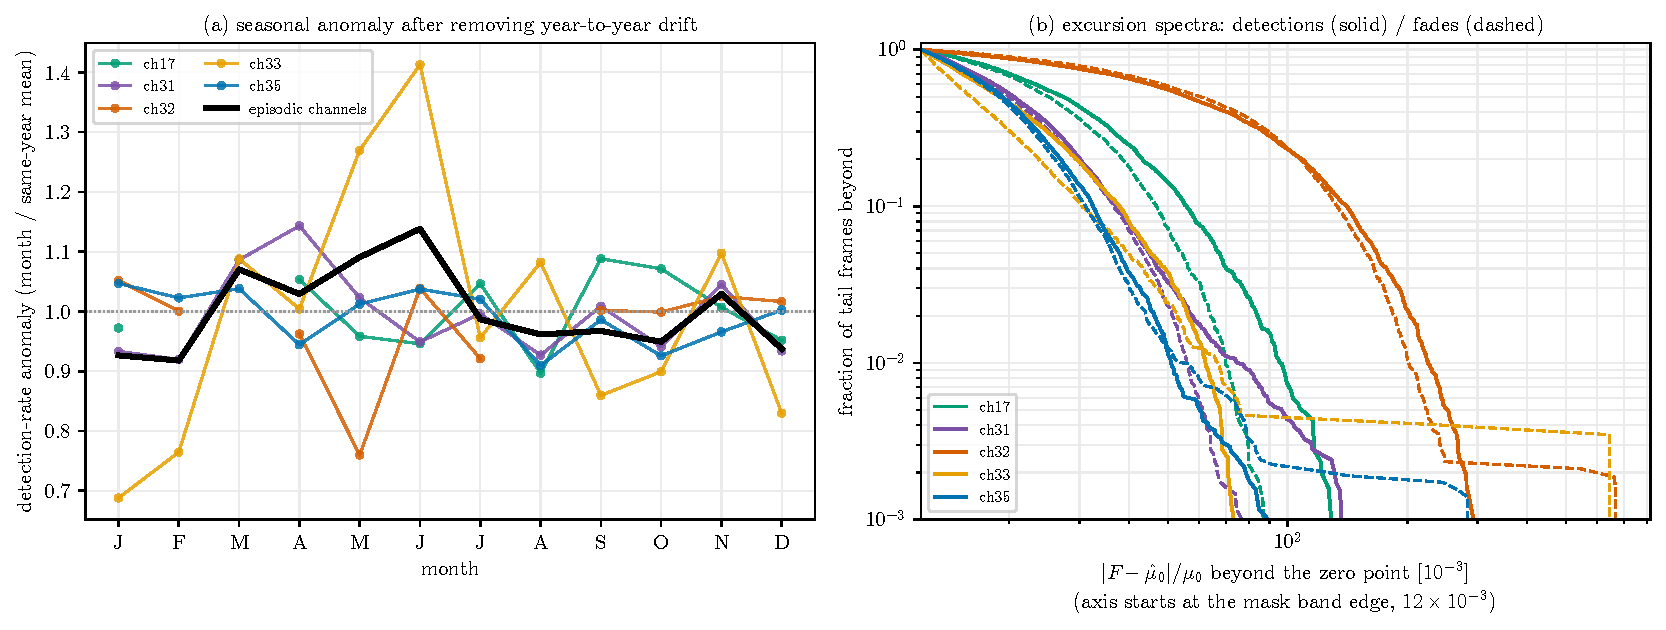
\includegraphics[width=\columnwidth]{fig_seasonal_propagation}
  \caption{(a) Seasonal detection-rate anomaly (month over same-year
  mean) after removing year-to-year secular drift, per episodic channel
  (the Fig.~7 set) and their aggregate (black): $\le 1.24\times$ peak-to-trough and not
  coherent across channels (Section~\ref{sec:secular}). (b) Excursion
  spectra of tail frames --- the fraction beyond a given
  $|F-\hat\mu_0|/\mu_0$, detections (solid) and fades (dashed); the axis
  begins at the mask band edge ($12\times10^{-3}$).
  \label{fig:seasonal}}
\end{figure}

\FloatBarrier  % keep Fig. 10 with Appendix A, ahead of Appendix B
\section{Recorded analysis choices and the stack subset}
\label{app:prereg}
The combine rule was recorded 2026-07-08 and amended 2026-07-14 to
``maximize common events subject to a $\ge$16-channel floor,''
implemented as a \emph{signature-seeded heuristic}: an exact per-block
search over the observed event-presence signatures, each candidate
closed to the intersection of its covering signatures --- exact per
block, but not an unrestricted maximization. This recorded procedure
selects \textbf{16
channels $\times$ 1548 common events} (physical channels 14, 16--19,
21, 22, 25, 27--29, 31, 33--36). Event-keyed alignment retains 1329 of
these events (5638 frames): the combine stacks frames by (event,
frame-in-file) identity, so the 219 events whose per-channel captures
differ in frame count or alignment drop out even though all 16 channels
observed them. The procedure was re-run end-to-end on 2026-07-17
against the complete product snapshot (77\,423 channel--event pairs,
matching Section~\ref{sec:survey} exactly; integrity pass on all 23
products) and reproduces the same selection, which the stacked
analyses use. For completeness we record that an \emph{unrestricted}
exhaustive search over all $\binom{23}{16}$ channel subsets finds a
larger block --- 1829 common events on channels 15--23, 25, 27--29, 33,
34, 36 --- that signature-seeded candidates structurally cannot reach
(the seeded table is not even monotone in $k$); we retain the
procedure-as-recorded selection and did not adopt the larger block.
Robustness across blocks (measured, 2026-07-17): re-running the full
pipeline with the unrestricted block as an explicit amendment yields the
same 1829 presence-common events by the pipeline's own count, aligning
to 1611 events (6890 frames), stack-level $\mathcal{H}_0$ tracking on
10/16 channels (vs 8/16), and a stacked recovered-bandwidth headline of
3.53 vs 3.74\,MHz of 6.25 --- a composition effect of the three-channel
swap (the recorded block includes ch14, mask fraction 0.090), not an
instability. Per-channel and full-depth quantities are block-independent
(4.71 of 8.98\,MHz unchanged); no stacked conclusion in this paper
depends on the block choice. Both runs' decision records are archived. The
registered greedy rule strands at 22 channels $\times$ 12 events on the
same data. The recorded procedure's by-$k$ table and drop-curve, and
the unrestricted by-$k$ table, are archived
(\texttt{appendix\_exact\_by\_k.csv}, \texttt{appendix\_dropcurve.csv},
\texttt{appendix\_unrestricted\_by\_k.csv}, from
\texttt{event\_presence\_signatures.npz} and
\texttt{combine\_subset\_decision.json}). We describe these as recorded
analysis choices rather than preregistration. \needsdylan{confirm which
choices were recorded before inspecting any relevant outcome (e.g.,
whether the 07-14 amendment postdated the drop curve); wording may be
strengthened for those that were.}

\section{Exact-integer threshold constants}
\label{app:constants}
The measured ceiling and floor are shipped as per-channel rational pairs
$(P, Q)$, $Q \le 2^{16}$: mask$_{\rm hi}$ iff $P_t Q > P\,P_r$ and
mask$_{\rm lo}$ iff $P_t Q_{\rm lo} < P_{\rm lo} P_r$. Approximation error
is $\le 10^{-9}$ (four orders below the zero points' statistical error);
verification against the float rules disagrees on 0 of 339\,196 frames;
worst product width 55 bits. Full table:
\texttt{empirical\_thresholds.csv}.

\section{Reproducibility}
\label{app:repro}
Every number in this paper maps to a command in the repository
(\texttt{analysis/README.md}); the analysis plan
(\texttt{docs/PAPER\_PLAN.md}) records the figure inventory and
decisions, and the CI suite includes the Monte-Carlo zero-point gate
(\texttt{tests/core/test\_mask\_zero\_point.py}).


\end{document}
